% Options for packages loaded elsewhere
\PassOptionsToPackage{unicode}{hyperref}
\PassOptionsToPackage{hyphens}{url}
%
\documentclass[
  11pt,
]{article}
\usepackage{amsmath,amssymb}
\usepackage{iftex}
\ifPDFTeX
  \usepackage[T1]{fontenc}
  \usepackage[utf8]{inputenc}
  \usepackage{textcomp} % provide euro and other symbols
\else % if luatex or xetex
  \usepackage{unicode-math} % this also loads fontspec
  \defaultfontfeatures{Scale=MatchLowercase}
  \defaultfontfeatures[\rmfamily]{Ligatures=TeX,Scale=1}
\fi
\usepackage{lmodern}
\ifPDFTeX\else
  % xetex/luatex font selection
    \setmainfont[]{Times New Roman}
    \setmonofont[]{Courier New}
\fi
% Use upquote if available, for straight quotes in verbatim environments
\IfFileExists{upquote.sty}{\usepackage{upquote}}{}
\IfFileExists{microtype.sty}{% use microtype if available
  \usepackage[]{microtype}
  \UseMicrotypeSet[protrusion]{basicmath} % disable protrusion for tt fonts
}{}
\makeatletter
\@ifundefined{KOMAClassName}{% if non-KOMA class
  \IfFileExists{parskip.sty}{%
    \usepackage{parskip}
  }{% else
    \setlength{\parindent}{0pt}
    \setlength{\parskip}{6pt plus 2pt minus 1pt}}
}{% if KOMA class
  \KOMAoptions{parskip=half}}
\makeatother
\usepackage{xcolor}
\usepackage[margin=1in]{geometry}
\usepackage{color}
\usepackage{fancyvrb}
\newcommand{\VerbBar}{|}
\newcommand{\VERB}{\Verb[commandchars=\\\{\}]}
\DefineVerbatimEnvironment{Highlighting}{Verbatim}{commandchars=\\\{\}}
% Add ',fontsize=\small' for more characters per line
\usepackage{framed}
\definecolor{shadecolor}{RGB}{248,248,248}
\newenvironment{Shaded}{\begin{snugshade}}{\end{snugshade}}
\newcommand{\AlertTok}[1]{\textcolor[rgb]{0.94,0.16,0.16}{#1}}
\newcommand{\AnnotationTok}[1]{\textcolor[rgb]{0.56,0.35,0.01}{\textbf{\textit{#1}}}}
\newcommand{\AttributeTok}[1]{\textcolor[rgb]{0.13,0.29,0.53}{#1}}
\newcommand{\BaseNTok}[1]{\textcolor[rgb]{0.00,0.00,0.81}{#1}}
\newcommand{\BuiltInTok}[1]{#1}
\newcommand{\CharTok}[1]{\textcolor[rgb]{0.31,0.60,0.02}{#1}}
\newcommand{\CommentTok}[1]{\textcolor[rgb]{0.56,0.35,0.01}{\textit{#1}}}
\newcommand{\CommentVarTok}[1]{\textcolor[rgb]{0.56,0.35,0.01}{\textbf{\textit{#1}}}}
\newcommand{\ConstantTok}[1]{\textcolor[rgb]{0.56,0.35,0.01}{#1}}
\newcommand{\ControlFlowTok}[1]{\textcolor[rgb]{0.13,0.29,0.53}{\textbf{#1}}}
\newcommand{\DataTypeTok}[1]{\textcolor[rgb]{0.13,0.29,0.53}{#1}}
\newcommand{\DecValTok}[1]{\textcolor[rgb]{0.00,0.00,0.81}{#1}}
\newcommand{\DocumentationTok}[1]{\textcolor[rgb]{0.56,0.35,0.01}{\textbf{\textit{#1}}}}
\newcommand{\ErrorTok}[1]{\textcolor[rgb]{0.64,0.00,0.00}{\textbf{#1}}}
\newcommand{\ExtensionTok}[1]{#1}
\newcommand{\FloatTok}[1]{\textcolor[rgb]{0.00,0.00,0.81}{#1}}
\newcommand{\FunctionTok}[1]{\textcolor[rgb]{0.13,0.29,0.53}{\textbf{#1}}}
\newcommand{\ImportTok}[1]{#1}
\newcommand{\InformationTok}[1]{\textcolor[rgb]{0.56,0.35,0.01}{\textbf{\textit{#1}}}}
\newcommand{\KeywordTok}[1]{\textcolor[rgb]{0.13,0.29,0.53}{\textbf{#1}}}
\newcommand{\NormalTok}[1]{#1}
\newcommand{\OperatorTok}[1]{\textcolor[rgb]{0.81,0.36,0.00}{\textbf{#1}}}
\newcommand{\OtherTok}[1]{\textcolor[rgb]{0.56,0.35,0.01}{#1}}
\newcommand{\PreprocessorTok}[1]{\textcolor[rgb]{0.56,0.35,0.01}{\textit{#1}}}
\newcommand{\RegionMarkerTok}[1]{#1}
\newcommand{\SpecialCharTok}[1]{\textcolor[rgb]{0.81,0.36,0.00}{\textbf{#1}}}
\newcommand{\SpecialStringTok}[1]{\textcolor[rgb]{0.31,0.60,0.02}{#1}}
\newcommand{\StringTok}[1]{\textcolor[rgb]{0.31,0.60,0.02}{#1}}
\newcommand{\VariableTok}[1]{\textcolor[rgb]{0.00,0.00,0.00}{#1}}
\newcommand{\VerbatimStringTok}[1]{\textcolor[rgb]{0.31,0.60,0.02}{#1}}
\newcommand{\WarningTok}[1]{\textcolor[rgb]{0.56,0.35,0.01}{\textbf{\textit{#1}}}}
\usepackage{graphicx}
\makeatletter
\newsavebox\pandoc@box
\newcommand*\pandocbounded[1]{% scales image to fit in text height/width
  \sbox\pandoc@box{#1}%
  \Gscale@div\@tempa{\textheight}{\dimexpr\ht\pandoc@box+\dp\pandoc@box\relax}%
  \Gscale@div\@tempb{\linewidth}{\wd\pandoc@box}%
  \ifdim\@tempb\p@<\@tempa\p@\let\@tempa\@tempb\fi% select the smaller of both
  \ifdim\@tempa\p@<\p@\scalebox{\@tempa}{\usebox\pandoc@box}%
  \else\usebox{\pandoc@box}%
  \fi%
}
% Set default figure placement to htbp
\def\fps@figure{htbp}
\makeatother
\setlength{\emergencystretch}{3em} % prevent overfull lines
\providecommand{\tightlist}{%
  \setlength{\itemsep}{0pt}\setlength{\parskip}{0pt}}
\setcounter{secnumdepth}{5}

% Preamble for DRD Final Report PDF output
\usepackage{fancyvrb}
\usepackage{fvextra}
\usepackage{geometry}
\usepackage{titlesec}
\usepackage{longtable}
\usepackage{caption}
\usepackage{fontspec}
\setmainfont{Times New Roman}

% Better handling of long code lines
\DefineVerbatimEnvironment{Highlighting}{Verbatim}
{breaklines, breakanywhere, fontsize=\small, commandchars=\\\{\}}

% Prevent code from overflowing page margins
\fvset{breaklines=true, breakanywhere=true, fontsize=\small}

% Nicer table captioning
\captionsetup[table]{skip=10pt}

% Tighten sections a bit
\titlespacing*{\section}{0pt}{*2}{*1}
\titlespacing*{\subsection}{0pt}{*2}{*1}
\titlespacing*{\subsubsection}{0pt}{*2}{*1}
\usepackage{bookmark}
\IfFileExists{xurl.sty}{\usepackage{xurl}}{} % add URL line breaks if available
\urlstyle{same}
\hypersetup{
  pdftitle={Comprehensive Analysis of DNA Methylation Using the Illumina HumanMethylation450 BeadChip Platform},
  pdfauthor={Keshani, K., Castro Vargas, P., Gustini, B., Aynede, A., Dobrokhotov, I., \& Otoijamun, F.},
  hidelinks,
  pdfcreator={LaTeX via pandoc}}

\title{Comprehensive Analysis of DNA Methylation Using the Illumina
HumanMethylation450 BeadChip Platform}
\author{Keshani, K., Castro Vargas, P., Gustini, B., Aynede, A.,
Dobrokhotov, I., \& Otoijamun, F.}
\date{2025-06}

\begin{document}
\maketitle

{
\setcounter{tocdepth}{3}
\tableofcontents
}
Keshani, K., Castro Vargas, P., Gustini, B., MohammadNejad Aynede, A.,
Dobrokhotov, I., \& Otoijamun, F. (2025). DRD\_2025\_Project:
Educational pipeline for DNA methylation analysis (Version 1.0.0)
{[}Computer software{]}.
\url{https://github.com/kianinsilico/DRD_2025_Project}

\section{Introduction}\label{introduction}

This project focuses on the analysis of DNA methylation data generated
using the Illumina HumanMethylation450 BeadChip (450K array) to explore
epigenetic differences between sample groups. Utilizing statistical
tests, principal component analysis, and heatmap visualizations, the
study aims to identify significant methylation patterns that may
contribute to biological insights. This work was conducted as part of
the DNA/RNA Dynamics course at the Università di Bologna, combining
practical bioinformatics techniques with real epigenomic datasets to
deepen understanding of epigenetic regulation mechanisms.

\section{Analytical pipeline and R
code}\label{analytical-pipeline-and-r-code}

\subsection{STEP 0. BASIC PREPARATION (Environment Setting and Importing
Libraries)}\label{step-0.-basic-preparation-environment-setting-and-importing-libraries}

\textbf{Set the proper working directory where the data is stored}

\begin{Shaded}
\begin{Highlighting}[]
\CommentTok{\#setwd("\textasciitilde{}/DRD\_2025\_Project")}
\end{Highlighting}
\end{Shaded}

\textbf{Install and load the necessary packages}

\begin{Shaded}
\begin{Highlighting}[]
\FunctionTok{library}\NormalTok{(minfi)}
\FunctionTok{library}\NormalTok{(minfiData)}
\FunctionTok{library}\NormalTok{(IlluminaHumanMethylation450kmanifest)}
\FunctionTok{library}\NormalTok{(IlluminaHumanMethylation450kanno.ilmn12.hg19)}
\FunctionTok{library}\NormalTok{(shinyMethyl)}
\FunctionTok{library}\NormalTok{(AnnotationDbi)}
\FunctionTok{library}\NormalTok{(sva)}
\FunctionTok{library}\NormalTok{(gplots)}
\FunctionTok{library}\NormalTok{(qqman)}
\FunctionTok{library}\NormalTok{(tinytex)}
\FunctionTok{install.packages}\NormalTok{(}\StringTok{"../lib/SummarizedExperiment\_1.38.0.tar.gz"}\NormalTok{, }\AttributeTok{repos =} \ConstantTok{NULL}\NormalTok{)}
\end{Highlighting}
\end{Shaded}

\subsection{STEP 1. DATA IMPORT AND OBJECT
CREATION}\label{step-1.-data-import-and-object-creation}

Load raw data with minfi and create an object called RGset storing the
RGChannelSet object.

\textbf{List files in data directory}

\begin{Shaded}
\begin{Highlighting}[]
\FunctionTok{list.files}\NormalTok{(}\StringTok{"../data/raw/"}\NormalTok{)}
\end{Highlighting}
\end{Shaded}

\textbf{Load the sample sheet}

\begin{Shaded}
\begin{Highlighting}[]
\NormalTok{SampleSheet }\OtherTok{\textless{}{-}} \FunctionTok{read.csv}\NormalTok{(}\StringTok{"../data/raw/SampleSheet\_Report\_II.csv"}\NormalTok{, }\AttributeTok{header =} \ConstantTok{TRUE}\NormalTok{)}
\NormalTok{SampleSheet}
\end{Highlighting}
\end{Shaded}

\textbf{Load sample sheet using minfi's function}

\begin{Shaded}
\begin{Highlighting}[]
\NormalTok{baseDir }\OtherTok{\textless{}{-}}\NormalTok{ (}\StringTok{"../data/raw"}\NormalTok{)}
\NormalTok{targets }\OtherTok{\textless{}{-}} \FunctionTok{read.metharray.sheet}\NormalTok{(baseDir)}
\NormalTok{targets}
\end{Highlighting}
\end{Shaded}

\textbf{Create RGChannelSet object}

\begin{Shaded}
\begin{Highlighting}[]
\NormalTok{RGset }\OtherTok{\textless{}{-}} \FunctionTok{read.metharray.exp}\NormalTok{(}\AttributeTok{targets =}\NormalTok{ targets)}
\FunctionTok{save}\NormalTok{(RGset, }\AttributeTok{file =} \StringTok{"../data/processed/RGChannelSet.RData"}\NormalTok{)}
\FunctionTok{load}\NormalTok{(}\StringTok{"../data/processed/RGChannelSet.RData"}\NormalTok{)}
\end{Highlighting}
\end{Shaded}

\textbf{Explore the RGset object}

\begin{Shaded}
\begin{Highlighting}[]
\NormalTok{RGset}
\end{Highlighting}
\end{Shaded}

\begin{Shaded}
\begin{Highlighting}[]
\FunctionTok{str}\NormalTok{(RGset)}
\end{Highlighting}
\end{Shaded}

\subsection{STEP 2. EXTRACT RED AND GREEN
CHANNELS}\label{step-2.-extract-red-and-green-channels}

Create dataframes to store the red and green fluorescences.

\textbf{Extract fluorescence intensity information for Red and Green
channels}

\begin{Shaded}
\begin{Highlighting}[]
\NormalTok{Red }\OtherTok{\textless{}{-}} \FunctionTok{data.frame}\NormalTok{(}\FunctionTok{getRed}\NormalTok{(RGset))}
\FunctionTok{dim}\NormalTok{(Red)}
\FunctionTok{head}\NormalTok{(Red)}
\NormalTok{Green }\OtherTok{\textless{}{-}} \FunctionTok{data.frame}\NormalTok{(}\FunctionTok{getGreen}\NormalTok{(RGset))}
\FunctionTok{dim}\NormalTok{(Green)}
\FunctionTok{head}\NormalTok{(Green)}
\end{Highlighting}
\end{Shaded}

\subsection{STEP 3. PROBE INFORMATION AND ADDRESS
CHECKS}\label{step-3.-probe-information-and-address-checks}

Determine whether address 18756452 belongs to a Type I or Type II probe
by retrieving the red and green fluorescence values for this address and
checking the manifest file.

\textbf{Explore manifest and probe information}

\begin{Shaded}
\begin{Highlighting}[]
\FunctionTok{getManifest}\NormalTok{(RGset)}
\FunctionTok{getManifestInfo}\NormalTok{(RGset)}
\FunctionTok{getProbeInfo}\NormalTok{(RGset)}
\NormalTok{ProbeInfo\_I }\OtherTok{\textless{}{-}} \FunctionTok{data.frame}\NormalTok{(}\FunctionTok{getProbeInfo}\NormalTok{(RGset))}
\FunctionTok{dim}\NormalTok{(ProbeInfo\_I)}
\FunctionTok{head}\NormalTok{(}\FunctionTok{getProbeInfo}\NormalTok{(RGset, }\AttributeTok{type =} \StringTok{"II"}\NormalTok{))}
\NormalTok{ProbeInfo\_II }\OtherTok{\textless{}{-}} \FunctionTok{data.frame}\NormalTok{(}\FunctionTok{getProbeInfo}\NormalTok{(RGset, }\AttributeTok{type =} \StringTok{"II"}\NormalTok{))}
\FunctionTok{dim}\NormalTok{(ProbeInfo\_II)}
\end{Highlighting}
\end{Shaded}

\textbf{Check probe with address 18756452}

\begin{Shaded}
\begin{Highlighting}[]
\NormalTok{ProbeInfo\_I[ProbeInfo\_I}\SpecialCharTok{$}\NormalTok{AddressA }\SpecialCharTok{==} \StringTok{"18756452"}\NormalTok{,]}
\NormalTok{ProbeInfo\_I[ProbeInfo\_I}\SpecialCharTok{$}\NormalTok{AddressB }\SpecialCharTok{==} \StringTok{"18756452"}\NormalTok{,]}
\NormalTok{ProbeInfo\_II[ProbeInfo\_II}\SpecialCharTok{$}\NormalTok{AddressB }\SpecialCharTok{==} \StringTok{"18756452"}\NormalTok{,]}
\NormalTok{ProbeInfo\_II[ProbeInfo\_II}\SpecialCharTok{$}\NormalTok{AddressA }\SpecialCharTok{==} \StringTok{"18756452"}\NormalTok{,]}
\end{Highlighting}
\end{Shaded}

There is a Type II probe at address 18756452, identified by the name
cg01523029.

\textbf{Extract Red/Green fluorescence for address 18756452}

\begin{Shaded}
\begin{Highlighting}[]
\NormalTok{Probe\_Info\_18756452 }\OtherTok{\textless{}{-}}\NormalTok{ ProbeInfo\_II[ProbeInfo\_II}\SpecialCharTok{$}\NormalTok{AddressA }\SpecialCharTok{==} \StringTok{"18756452"}\NormalTok{,]}
\NormalTok{Red\_fluorescences }\OtherTok{\textless{}{-}}\NormalTok{ Red[}\FunctionTok{rownames}\NormalTok{(Red) }\SpecialCharTok{==} \StringTok{"18756452"}\NormalTok{,]}
\NormalTok{Green\_fluorescences }\OtherTok{\textless{}{-}}\NormalTok{ Green[}\FunctionTok{rownames}\NormalTok{(Green) }\SpecialCharTok{==} \StringTok{"18756452"}\NormalTok{,]}
\end{Highlighting}
\end{Shaded}

\textbf{Use sample names from the column names of Red/Green (same order)
and create summary dataframe to fill the requested table}

\begin{Shaded}
\begin{Highlighting}[]
\NormalTok{sample\_names }\OtherTok{\textless{}{-}} \FunctionTok{colnames}\NormalTok{(Red\_fluorescences)}
\NormalTok{df\_summary\_probes }\OtherTok{\textless{}{-}} \FunctionTok{data.frame}\NormalTok{(}
  \StringTok{"Sample"} \OtherTok{=}\NormalTok{ sample\_names,}
  \StringTok{"Red Fluorescence"} \OtherTok{=} \FunctionTok{as.numeric}\NormalTok{ (Red\_fluorescences[}\DecValTok{1}\NormalTok{, ]),}
  \StringTok{"Green Fluorescence"} \OtherTok{=} \FunctionTok{as.numeric}\NormalTok{ (Green\_fluorescences[}\DecValTok{1}\NormalTok{,]),}
  \StringTok{"Type"} \OtherTok{=} \FunctionTok{rep}\NormalTok{(}\StringTok{"II"}\NormalTok{, }\FunctionTok{length}\NormalTok{(sample\_names)),}
  \StringTok{"Color"} \OtherTok{=} \FunctionTok{rep}\NormalTok{(}\StringTok{"Both"}\NormalTok{, }\FunctionTok{length}\NormalTok{(sample\_names))}
\NormalTok{)}
\FunctionTok{print}\NormalTok{(df\_summary\_probes)}
\end{Highlighting}
\end{Shaded}

\subsection{STEP 4. Creation of the MSet.raw
oject}\label{step-4.-creation-of-the-mset.raw-oject}

\textbf{Extract methylated and unmethylated signals}

\begin{Shaded}
\begin{Highlighting}[]
\NormalTok{MSet.raw }\OtherTok{\textless{}{-}} \FunctionTok{preprocessRaw}\NormalTok{(RGset)}
\NormalTok{MSet.raw}
\FunctionTok{save}\NormalTok{(MSet.raw, }\AttributeTok{file =} \StringTok{"../data/processed/MSet\_raw.RData"}\NormalTok{)}
\NormalTok{Meth }\OtherTok{\textless{}{-}} \FunctionTok{as.matrix}\NormalTok{(}\FunctionTok{getMeth}\NormalTok{(MSet.raw))}
\FunctionTok{str}\NormalTok{(Meth)}
\FunctionTok{head}\NormalTok{(Meth)}
\NormalTok{Unmeth }\OtherTok{\textless{}{-}} \FunctionTok{as.matrix}\NormalTok{(}\FunctionTok{getUnmeth}\NormalTok{(MSet.raw))}
\FunctionTok{str}\NormalTok{(Unmeth)}
\FunctionTok{head}\NormalTok{(Unmeth)}
\end{Highlighting}
\end{Shaded}

\textbf{Check probe cg01523029 in MethylSet}

\begin{Shaded}
\begin{Highlighting}[]
\NormalTok{Unmeth[}\FunctionTok{rownames}\NormalTok{(Unmeth) }\SpecialCharTok{==} \StringTok{"cg01523029"}\NormalTok{,]}
\NormalTok{Meth[}\FunctionTok{rownames}\NormalTok{(Meth) }\SpecialCharTok{==} \StringTok{"cg01523029"}\NormalTok{,]}

\FunctionTok{load}\NormalTok{(}\StringTok{"../data/raw/Illumina450Manifest.RData"}\NormalTok{)}
\NormalTok{Illumina450Manifest\_clean }\OtherTok{\textless{}{-}}\NormalTok{ Illumina450Manifest[Illumina450Manifest}\SpecialCharTok{$}\NormalTok{CHR }\SpecialCharTok{!=} \StringTok{""}\NormalTok{,]}
\NormalTok{Illumina450Manifest\_clean }\OtherTok{\textless{}{-}} \FunctionTok{droplevels}\NormalTok{(Illumina450Manifest\_clean)}
\NormalTok{Probe\_Info\_cg01523029 }\OtherTok{\textless{}{-}}\NormalTok{ Illumina450Manifest\_clean[Illumina450Manifest\_clean}\SpecialCharTok{$}\NormalTok{IlmnID }\SpecialCharTok{==} \StringTok{"cg01523029"}\NormalTok{,]}
\end{Highlighting}
\end{Shaded}

\subsection{5. Quality control}\label{quality-control}

Perform quality checks and provide a brief comment to each step.

\subsubsection{a. QCplot}\label{a.-qcplot}

\begin{Shaded}
\begin{Highlighting}[]
\NormalTok{qc }\OtherTok{\textless{}{-}} \FunctionTok{getQC}\NormalTok{(MSet.raw)}
\NormalTok{qc}
\end{Highlighting}
\end{Shaded}

\begin{verbatim}
## DataFrame with 8 rows and 2 columns
##                                     mMed      uMed
##                                <numeric> <numeric>
## GSM5319592_200121140049_R01C02  10.26327   9.76321
## GSM5319603_3999356129_R02C02     8.62205   8.82018
## GSM5319604_3999547012_R02C01    10.35094  10.23721
## GSM5319607_3999547012_R03C02    10.79360  10.90313
## GSM5319609_3999547016_R02C01     8.82655   8.83289
## GSM5319613_3999547017_R02C01    10.83684  10.69523
## GSM5319615_3999547017_R04C01    11.15038  11.04644
## GSM5319616_3999547017_R06C01    10.27845  10.33316
\end{verbatim}

\begin{Shaded}
\begin{Highlighting}[]
\FunctionTok{plotQC}\NormalTok{(qc)}
\end{Highlighting}
\end{Shaded}

\pandocbounded{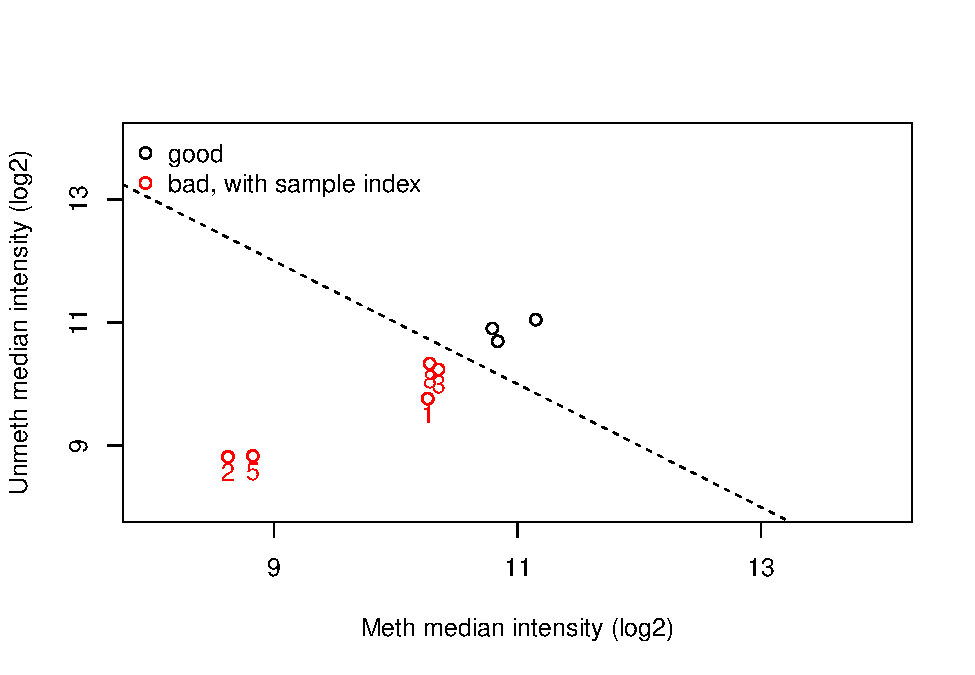
\includegraphics[keepaspectratio]{../results/QCplot-1.pdf}}

\textbf{Comment:} A QC plot displays the distribution of methylated and
unmethylated signal medians. High median values for both signals
indicate high-quality data. In this case, the samples are spread apart,
and most show low median values for both signals, suggesting poor
quality. Out of the eight samples, only three are considered to be of
good quality.

\subsubsection{b. Check the intensity of negative
controls}\label{b.-check-the-intensity-of-negative-controls}

\begin{Shaded}
\begin{Highlighting}[]
\NormalTok{NegativeControl }\OtherTok{\textless{}{-}} \FunctionTok{data.frame}\NormalTok{(}\FunctionTok{getProbeInfo}\NormalTok{(RGset, }\AttributeTok{type =} \StringTok{"Control"}\NormalTok{))}
\FunctionTok{table}\NormalTok{(NegativeControl}\SpecialCharTok{$}\NormalTok{Type)}
\end{Highlighting}
\end{Shaded}

\begin{verbatim}
## 
##  BISULFITE CONVERSION I BISULFITE CONVERSION II               EXTENSION 
##                      12                       4                       4 
##           HYBRIDIZATION                NEGATIVE         NON-POLYMORPHIC 
##                       3                     613                       4 
##                  NORM_A                  NORM_C                  NORM_G 
##                      32                      61                      32 
##                  NORM_T             RESTORATION           SPECIFICITY I 
##                      61                       1                      12 
##          SPECIFICITY II                STAINING          TARGET REMOVAL 
##                       3                       4                       2
\end{verbatim}

\begin{Shaded}
\begin{Highlighting}[]
\FunctionTok{head}\NormalTok{(NegativeControl) }
\end{Highlighting}
\end{Shaded}

\begin{verbatim}
##    Address      Type  Color  ExtendedType
## 1 27630314  STAINING    Red    DNP (High)
## 2 43603326  STAINING Purple     DNP (Bkg)
## 3 41666334  STAINING  Green Biotin (High)
## 4 34648333  STAINING   Blue  Biotin (Bkg)
## 5 63642461 EXTENSION    Red Extension (A)
## 6 47640365 EXTENSION Purple Extension (T)
\end{verbatim}

\begin{Shaded}
\begin{Highlighting}[]
\FunctionTok{controlStripPlot}\NormalTok{(RGset, }\AttributeTok{controls =} \StringTok{"NEGATIVE"}\NormalTok{)}
\end{Highlighting}
\end{Shaded}

\pandocbounded{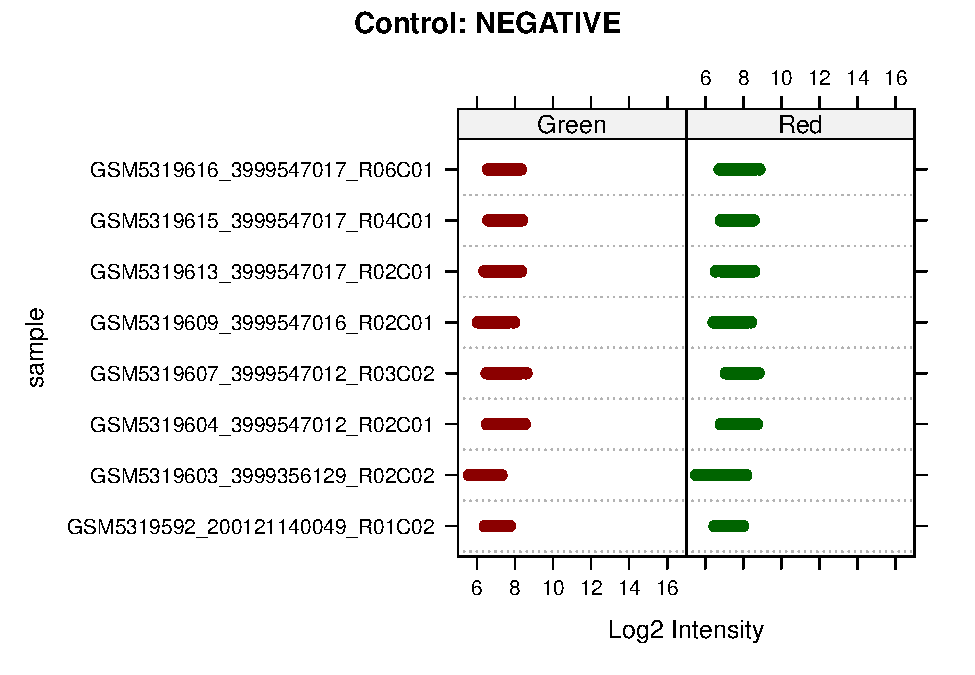
\includegraphics[keepaspectratio]{../results/NegativeControlIntesity-1.pdf}}

\textbf{Comment:} In this case, the negative control signals show
intensity values (log2) below 10 in both the red and green channels,
which is considered acceptable.

\subsubsection{c.~Calculation of detection
p-values}\label{c.-calculation-of-detection-p-values}

\begin{Shaded}
\begin{Highlighting}[]
\NormalTok{Detection\_pvalue }\OtherTok{\textless{}{-}} \FunctionTok{detectionP}\NormalTok{(RGset)}
\FunctionTok{save}\NormalTok{(Detection\_pvalue, }\AttributeTok{file =} \StringTok{"../data/processed/Detection\_pvalue.RData"}\NormalTok{)}
\NormalTok{Over\_Threshold }\OtherTok{\textless{}{-}}\NormalTok{ Detection\_pvalue }\SpecialCharTok{\textgreater{}} \FloatTok{0.05}
\FunctionTok{head}\NormalTok{(Over\_Threshold)}
\end{Highlighting}
\end{Shaded}

\begin{verbatim}
##            GSM5319592_200121140049_R01C02 GSM5319603_3999356129_R02C02
## cg00050873                          FALSE                        FALSE
## cg00212031                          FALSE                        FALSE
## cg00213748                          FALSE                        FALSE
## cg00214611                          FALSE                        FALSE
## cg00455876                          FALSE                        FALSE
## cg01707559                          FALSE                        FALSE
##            GSM5319604_3999547012_R02C01 GSM5319607_3999547012_R03C02
## cg00050873                        FALSE                        FALSE
## cg00212031                         TRUE                        FALSE
## cg00213748                        FALSE                        FALSE
## cg00214611                         TRUE                        FALSE
## cg00455876                        FALSE                        FALSE
## cg01707559                        FALSE                        FALSE
##            GSM5319609_3999547016_R02C01 GSM5319613_3999547017_R02C01
## cg00050873                        FALSE                        FALSE
## cg00212031                        FALSE                        FALSE
## cg00213748                         TRUE                         TRUE
## cg00214611                         TRUE                         TRUE
## cg00455876                        FALSE                        FALSE
## cg01707559                        FALSE                        FALSE
##            GSM5319615_3999547017_R04C01 GSM5319616_3999547017_R06C01
## cg00050873                         TRUE                        FALSE
## cg00212031                         TRUE                        FALSE
## cg00213748                         TRUE                         TRUE
## cg00214611                         TRUE                         TRUE
## cg00455876                        FALSE                        FALSE
## cg01707559                        FALSE                        FALSE
\end{verbatim}

\begin{Shaded}
\begin{Highlighting}[]
\FunctionTok{table}\NormalTok{(Over\_Threshold)}
\end{Highlighting}
\end{Shaded}

\begin{verbatim}
## Over_Threshold
##   FALSE    TRUE 
## 3877813    6283
\end{verbatim}

\begin{Shaded}
\begin{Highlighting}[]
\FunctionTok{sum}\NormalTok{(Over\_Threshold)}
\end{Highlighting}
\end{Shaded}

\begin{verbatim}
## [1] 6283
\end{verbatim}

\begin{Shaded}
\begin{Highlighting}[]
\NormalTok{failed\_probe\_message }\OtherTok{\textless{}{-}} \FunctionTok{sprintf}\NormalTok{(}
  \StringTok{"There are \%s failed probes with a detection p{-}value higher than 0.05"}\NormalTok{,}
  \FunctionTok{sum}\NormalTok{(Over\_Threshold)}
\NormalTok{)}
\NormalTok{Over\_Threshold\_Per\_Sample }\OtherTok{\textless{}{-}} \FunctionTok{colSums}\NormalTok{(Over\_Threshold)}
\NormalTok{Over\_Threshold\_Per\_Sample}
\end{Highlighting}
\end{Shaded}

\begin{verbatim}
## GSM5319592_200121140049_R01C02   GSM5319603_3999356129_R02C02 
##                            202                            306 
##   GSM5319604_3999547012_R02C01   GSM5319607_3999547012_R03C02 
##                           1156                            366 
##   GSM5319609_3999547016_R02C01   GSM5319613_3999547017_R02C01 
##                           2735                            460 
##   GSM5319615_3999547017_R04C01   GSM5319616_3999547017_R06C01 
##                            384                            674
\end{verbatim}

\begin{Shaded}
\begin{Highlighting}[]
\FunctionTok{summary}\NormalTok{(Over\_Threshold)}
\end{Highlighting}
\end{Shaded}

\begin{verbatim}
##  GSM5319592_200121140049_R01C02 GSM5319603_3999356129_R02C02
##  Mode :logical                  Mode :logical               
##  FALSE:485310                   FALSE:485206                
##  TRUE :202                      TRUE :306                   
##  GSM5319604_3999547012_R02C01 GSM5319607_3999547012_R03C02
##  Mode :logical                Mode :logical               
##  FALSE:484356                 FALSE:485146                
##  TRUE :1156                   TRUE :366                   
##  GSM5319609_3999547016_R02C01 GSM5319613_3999547017_R02C01
##  Mode :logical                Mode :logical               
##  FALSE:482777                 FALSE:485052                
##  TRUE :2735                   TRUE :460                   
##  GSM5319615_3999547017_R04C01 GSM5319616_3999547017_R06C01
##  Mode :logical                Mode :logical               
##  FALSE:485128                 FALSE:484838                
##  TRUE :384                    TRUE :674
\end{verbatim}

\begin{Shaded}
\begin{Highlighting}[]
\NormalTok{failed }\OtherTok{\textless{}{-}} \FunctionTok{data.frame}\NormalTok{(}
  \AttributeTok{Sample =} \FunctionTok{names}\NormalTok{(Over\_Threshold\_Per\_Sample),}
  \AttributeTok{n\_Failed\_Positions =}\NormalTok{ Over\_Threshold\_Per\_Sample}
\NormalTok{)}
\FunctionTok{print}\NormalTok{(failed)}
\end{Highlighting}
\end{Shaded}

\begin{verbatim}
##                                                        Sample
## GSM5319592_200121140049_R01C02 GSM5319592_200121140049_R01C02
## GSM5319603_3999356129_R02C02     GSM5319603_3999356129_R02C02
## GSM5319604_3999547012_R02C01     GSM5319604_3999547012_R02C01
## GSM5319607_3999547012_R03C02     GSM5319607_3999547012_R03C02
## GSM5319609_3999547016_R02C01     GSM5319609_3999547016_R02C01
## GSM5319613_3999547017_R02C01     GSM5319613_3999547017_R02C01
## GSM5319615_3999547017_R04C01     GSM5319615_3999547017_R04C01
## GSM5319616_3999547017_R06C01     GSM5319616_3999547017_R06C01
##                                n_Failed_Positions
## GSM5319592_200121140049_R01C02                202
## GSM5319603_3999356129_R02C02                  306
## GSM5319604_3999547012_R02C01                 1156
## GSM5319607_3999547012_R03C02                  366
## GSM5319609_3999547016_R02C01                 2735
## GSM5319613_3999547017_R02C01                  460
## GSM5319615_3999547017_R04C01                  384
## GSM5319616_3999547017_R06C01                  674
\end{verbatim}

\begin{Shaded}
\begin{Highlighting}[]
\FunctionTok{print}\NormalTok{(failed\_probe\_message)}
\end{Highlighting}
\end{Shaded}

\begin{verbatim}
## [1] "There are 6283 failed probes with a detection p-value higher than 0.05"
\end{verbatim}

\textbf{Comment:} There are 6283 failed probes with a detection p-value
higher than 0.05 and the number of failed positions ranges from 202-2735
per sample.

\subsection{STEP 6. Calculation of Beta and M values, Plot
Densities}\label{step-6.-calculation-of-beta-and-m-values-plot-densities}

Calculate raw beta and M values and plot the densities of mean
methylation values, dividing the samples in CTRL and DIS (suggestion:
subset the beta and M values matrixes in order to retain CTRL or DIS
subjects and apply the function mean to the 2 subsets).

\textbf{Data preparation}

\begin{Shaded}
\begin{Highlighting}[]
\NormalTok{beta }\OtherTok{\textless{}{-}} \FunctionTok{getBeta}\NormalTok{(MSet.raw)}
\NormalTok{M }\OtherTok{\textless{}{-}} \FunctionTok{getM}\NormalTok{(MSet.raw)}
\NormalTok{beta\_df }\OtherTok{\textless{}{-}} \FunctionTok{data.frame}\NormalTok{(beta)}
\NormalTok{M\_df }\OtherTok{\textless{}{-}} \FunctionTok{data.frame}\NormalTok{(M)}

\NormalTok{pheno }\OtherTok{\textless{}{-}} \FunctionTok{read.csv}\NormalTok{(}\StringTok{"../data/raw/SampleSheet\_Report\_II.csv"}\NormalTok{, }\AttributeTok{header =} \ConstantTok{TRUE}\NormalTok{, }\AttributeTok{stringsAsFactors =} \ConstantTok{TRUE}\NormalTok{)}

\NormalTok{SampleSheet}\SpecialCharTok{$}\NormalTok{Group}
\end{Highlighting}
\end{Shaded}

\begin{verbatim}
## [1] "CTRL" "DIS"  "DIS"  "CTRL" "DIS"  "DIS"  "CTRL" "CTRL"
\end{verbatim}

\begin{Shaded}
\begin{Highlighting}[]
\NormalTok{beta\_ctrl }\OtherTok{\textless{}{-}}\NormalTok{ beta\_df[SampleSheet}\SpecialCharTok{$}\NormalTok{Group }\SpecialCharTok{==} \StringTok{"CTRL"}\NormalTok{,]}
\NormalTok{beta\_dis }\OtherTok{\textless{}{-}}\NormalTok{ beta\_df[SampleSheet}\SpecialCharTok{$}\NormalTok{Group }\SpecialCharTok{==} \StringTok{"DIS"}\NormalTok{,]}
\NormalTok{M\_ctrl }\OtherTok{\textless{}{-}}\NormalTok{ M\_df[SampleSheet}\SpecialCharTok{$}\NormalTok{Group }\SpecialCharTok{==} \StringTok{"CTRL"}\NormalTok{,]}
\NormalTok{M\_dis }\OtherTok{\textless{}{-}}\NormalTok{ M\_df[SampleSheet}\SpecialCharTok{$}\NormalTok{Group }\SpecialCharTok{==} \StringTok{"DIS"}\NormalTok{,]}

\NormalTok{mean\_of\_beta\_ctrl }\OtherTok{\textless{}{-}} \FunctionTok{apply}\NormalTok{(beta\_ctrl, }\DecValTok{1}\NormalTok{, mean, }\AttributeTok{na.rm =} \ConstantTok{TRUE}\NormalTok{)}
\NormalTok{mean\_of\_beta\_dis }\OtherTok{\textless{}{-}} \FunctionTok{apply}\NormalTok{(beta\_dis, }\DecValTok{1}\NormalTok{, mean, }\AttributeTok{na.rm =} \ConstantTok{TRUE}\NormalTok{)}
\NormalTok{mean\_of\_M\_ctrl }\OtherTok{\textless{}{-}} \FunctionTok{apply}\NormalTok{(M\_ctrl, }\DecValTok{1}\NormalTok{, mean, }\AttributeTok{na.rm =} \ConstantTok{TRUE}\NormalTok{)}
\NormalTok{mean\_of\_M\_dis }\OtherTok{\textless{}{-}} \FunctionTok{apply}\NormalTok{(M\_dis, }\DecValTok{1}\NormalTok{, mean, }\AttributeTok{na.rm =} \ConstantTok{TRUE}\NormalTok{)}
\end{Highlighting}
\end{Shaded}

\textbf{Plotting the density of mean methylation values.}

\begin{Shaded}
\begin{Highlighting}[]
\NormalTok{plot\_density }\OtherTok{\textless{}{-}} \ControlFlowTok{function}\NormalTok{() \{}
  \FunctionTok{par}\NormalTok{(}\AttributeTok{mfrow =} \FunctionTok{c}\NormalTok{(}\DecValTok{1}\NormalTok{, }\DecValTok{2}\NormalTok{), }\AttributeTok{mar =} \FunctionTok{c}\NormalTok{(}\DecValTok{5}\NormalTok{, }\DecValTok{4}\NormalTok{, }\DecValTok{4}\NormalTok{, }\DecValTok{2}\NormalTok{))  }
  \FunctionTok{plot}\NormalTok{(}\FunctionTok{density}\NormalTok{(mean\_of\_beta\_ctrl, }\AttributeTok{na.rm =} \ConstantTok{TRUE}\NormalTok{), }\AttributeTok{main =} \StringTok{"Density of Beta Values"}\NormalTok{,}
       \AttributeTok{col =} \StringTok{"black"}\NormalTok{, }\AttributeTok{lwd =} \DecValTok{2}\NormalTok{)}
  \FunctionTok{lines}\NormalTok{(}\FunctionTok{density}\NormalTok{(mean\_of\_beta\_dis, }\AttributeTok{na.rm =} \ConstantTok{TRUE}\NormalTok{), }\AttributeTok{col =} \StringTok{"orange"}\NormalTok{, }\AttributeTok{lwd =} \DecValTok{2}\NormalTok{)}
  \FunctionTok{legend}\NormalTok{(}\StringTok{"top"}\NormalTok{, }\AttributeTok{legend =} \FunctionTok{c}\NormalTok{(}\StringTok{"CTL"}\NormalTok{, }\StringTok{"DIS"}\NormalTok{),}
         \AttributeTok{col =} \FunctionTok{c}\NormalTok{(}\StringTok{"black"}\NormalTok{, }\StringTok{"orange"}\NormalTok{), }\AttributeTok{lwd =} \DecValTok{2}\NormalTok{,}
         \AttributeTok{cex =} \FloatTok{0.9}\NormalTok{, }\AttributeTok{bty =} \StringTok{"n"}\NormalTok{, }\AttributeTok{inset =} \FunctionTok{c}\NormalTok{(}\SpecialCharTok{{-}}\FloatTok{0.01}\NormalTok{, }\SpecialCharTok{{-}}\FloatTok{0.01}\NormalTok{))}
  \FunctionTok{plot}\NormalTok{(}\FunctionTok{density}\NormalTok{(mean\_of\_M\_ctrl, }\AttributeTok{na.rm =} \ConstantTok{TRUE}\NormalTok{), }\AttributeTok{main =} \StringTok{"Density of M Values"}\NormalTok{, }\AttributeTok{col =} \StringTok{"black"}\NormalTok{, }\AttributeTok{lwd =} \DecValTok{2}\NormalTok{)}
  \FunctionTok{lines}\NormalTok{(}\FunctionTok{density}\NormalTok{(mean\_of\_M\_dis, }\AttributeTok{na.rm =} \ConstantTok{TRUE}\NormalTok{), }\AttributeTok{col =} \StringTok{"orange"}\NormalTok{, }\AttributeTok{lwd =} \DecValTok{2}\NormalTok{)}
  \FunctionTok{legend}\NormalTok{(}\StringTok{"topright"}\NormalTok{, }\AttributeTok{legend =} \FunctionTok{c}\NormalTok{(}\StringTok{"CTL"}\NormalTok{, }\StringTok{"DIS"}\NormalTok{),}
         \AttributeTok{col =} \FunctionTok{c}\NormalTok{(}\StringTok{"black"}\NormalTok{, }\StringTok{"orange"}\NormalTok{), }\AttributeTok{lwd =} \DecValTok{2}\NormalTok{,}
         \AttributeTok{cex =} \FloatTok{0.9}\NormalTok{, }\AttributeTok{bty =} \StringTok{"n"}\NormalTok{, }\AttributeTok{inset =} \FunctionTok{c}\NormalTok{(}\SpecialCharTok{{-}}\FloatTok{0.01}\NormalTok{, }\SpecialCharTok{{-}}\FloatTok{0.01}\NormalTok{))}
\NormalTok{\}}
\FunctionTok{plot\_density}\NormalTok{()}
\end{Highlighting}
\end{Shaded}

\pandocbounded{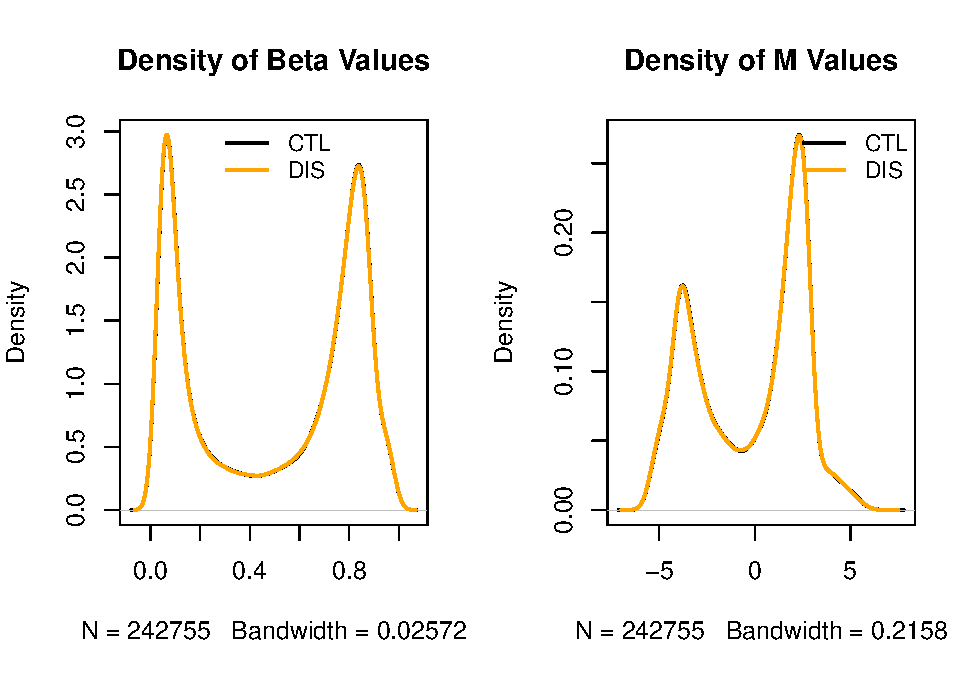
\includegraphics[keepaspectratio]{../results/MethylationValuesDensity-1.pdf}}

\textbf{Comment:} Based on the density plots of mean methylation, no
clear differences were observed between the control and disease groups.
This could suggest that there are no significant differences in
methylation levels between the two. However, further statistical
analyses are necessary to better interpret the data and potentially
uncover subtle or localized differences.

\subsection{STEP 7. Data normalization with
preprocessNoob}\label{step-7.-data-normalization-with-preprocessnoob}

Normalize the data using preprocessNoob and compare raw data and
normalized data. Produce a plot with 6 panels in which, for both raw and
normalized data, you show the density plots of beta mean values
according to the chemistry of the probes, the density plot of beta
standard deviation values according to the chemistry of the probes and
the boxplot of beta values.

\textbf{Subset beta values by probe type}

\begin{Shaded}
\begin{Highlighting}[]
\NormalTok{dfI }\OtherTok{\textless{}{-}}\NormalTok{ Illumina450Manifest\_clean[Illumina450Manifest\_clean}\SpecialCharTok{$}\NormalTok{Infinium\_Design\_Type }\SpecialCharTok{==} \StringTok{"I"}\NormalTok{,]}
\NormalTok{dfI }\OtherTok{\textless{}{-}} \FunctionTok{droplevels}\NormalTok{(dfI)}
\NormalTok{dfII }\OtherTok{\textless{}{-}}\NormalTok{ Illumina450Manifest\_clean[Illumina450Manifest\_clean}\SpecialCharTok{$}\NormalTok{Infinium\_Design\_Type }\SpecialCharTok{==} \StringTok{"II"}\NormalTok{,]}
\NormalTok{dfII }\OtherTok{\textless{}{-}} \FunctionTok{droplevels}\NormalTok{(dfII)}

\NormalTok{beta\_I }\OtherTok{\textless{}{-}}\NormalTok{ beta[}\FunctionTok{rownames}\NormalTok{(beta) }\SpecialCharTok{\%in\%}\NormalTok{ dfI}\SpecialCharTok{$}\NormalTok{IlmnID,]}
\NormalTok{beta\_II }\OtherTok{\textless{}{-}}\NormalTok{ beta[}\FunctionTok{rownames}\NormalTok{(beta) }\SpecialCharTok{\%in\%}\NormalTok{ dfII}\SpecialCharTok{$}\NormalTok{IlmnID,]}

\NormalTok{mean\_of\_beta\_I }\OtherTok{\textless{}{-}} \FunctionTok{apply}\NormalTok{(beta\_I, }\DecValTok{1}\NormalTok{, mean)}
\NormalTok{mean\_of\_beta\_II }\OtherTok{\textless{}{-}} \FunctionTok{apply}\NormalTok{(beta\_II, }\DecValTok{1}\NormalTok{, mean)}
\NormalTok{d\_mean\_of\_beta\_I }\OtherTok{\textless{}{-}} \FunctionTok{density}\NormalTok{(mean\_of\_beta\_I, }\AttributeTok{na.rm =} \ConstantTok{TRUE}\NormalTok{)}
\NormalTok{d\_mean\_of\_beta\_II }\OtherTok{\textless{}{-}} \FunctionTok{density}\NormalTok{(mean\_of\_beta\_II, }\AttributeTok{na.rm =} \ConstantTok{TRUE}\NormalTok{)}
\end{Highlighting}
\end{Shaded}

\textbf{Calculation of the densities of the standard deviations} This
can be calculated using the function sd():

\begin{Shaded}
\begin{Highlighting}[]
\NormalTok{sd\_of\_beta\_I }\OtherTok{\textless{}{-}} \FunctionTok{apply}\NormalTok{(beta\_I, }\DecValTok{1}\NormalTok{, sd, }\AttributeTok{na.rm =} \ConstantTok{TRUE}\NormalTok{)}
\NormalTok{sd\_of\_beta\_II }\OtherTok{\textless{}{-}} \FunctionTok{apply}\NormalTok{(beta\_II, }\DecValTok{1}\NormalTok{, sd, }\AttributeTok{na.rm =} \ConstantTok{TRUE}\NormalTok{)}
\NormalTok{d\_sd\_of\_beta\_I }\OtherTok{\textless{}{-}} \FunctionTok{density}\NormalTok{(sd\_of\_beta\_I,)}
\NormalTok{d\_sd\_of\_beta\_II }\OtherTok{\textless{}{-}} \FunctionTok{density}\NormalTok{(}\FunctionTok{na.omit}\NormalTok{(sd\_of\_beta\_II))}
\end{Highlighting}
\end{Shaded}

\textbf{Use of preprocessNoob} Preparation of the data.

\begin{Shaded}
\begin{Highlighting}[]
\NormalTok{preprocessNoob\_results }\OtherTok{\textless{}{-}} \FunctionTok{preprocessNoob}\NormalTok{(RGset)}
\NormalTok{beta\_preprocessNoob }\OtherTok{\textless{}{-}} \FunctionTok{getBeta}\NormalTok{(preprocessNoob\_results)}
\FunctionTok{save}\NormalTok{(beta\_preprocessNoob, }\AttributeTok{file =} \StringTok{"../data/processed/beta\_preprocessNoob.RData"}\NormalTok{)}
\end{Highlighting}
\end{Shaded}

Divide normalized beta matrix by probe type and calculate statistics.

\begin{Shaded}
\begin{Highlighting}[]
\NormalTok{beta\_preprocessNoob\_I }\OtherTok{\textless{}{-}}\NormalTok{ beta\_preprocessNoob[}\FunctionTok{rownames}\NormalTok{(beta\_preprocessNoob) }\SpecialCharTok{\%in\%}\NormalTok{ dfI}\SpecialCharTok{$}\NormalTok{IlmnID,]}
\NormalTok{beta\_preprocessNoob\_II }\OtherTok{\textless{}{-}}\NormalTok{ beta\_preprocessNoob[}\FunctionTok{rownames}\NormalTok{(beta\_preprocessNoob) }\SpecialCharTok{\%in\%}\NormalTok{ dfII}\SpecialCharTok{$}\NormalTok{IlmnID,]}
\NormalTok{mean\_of\_beta\_preprocessNoob\_I }\OtherTok{\textless{}{-}} \FunctionTok{apply}\NormalTok{(beta\_preprocessNoob\_I, }\DecValTok{1}\NormalTok{, mean)}
\NormalTok{mean\_of\_beta\_preprocessNoob\_II }\OtherTok{\textless{}{-}} \FunctionTok{apply}\NormalTok{(beta\_preprocessNoob\_II, }\DecValTok{1}\NormalTok{, mean)}
\NormalTok{d\_mean\_of\_beta\_preprocessNoob\_I }\OtherTok{\textless{}{-}} \FunctionTok{density}\NormalTok{(mean\_of\_beta\_preprocessNoob\_I, }\AttributeTok{na.rm =} \ConstantTok{TRUE}\NormalTok{)}
\NormalTok{d\_mean\_of\_beta\_preprocessNoob\_II }\OtherTok{\textless{}{-}} \FunctionTok{density}\NormalTok{(mean\_of\_beta\_preprocessNoob\_II, }\AttributeTok{na.rm =} \ConstantTok{TRUE}\NormalTok{)}
\NormalTok{sd\_of\_beta\_preprocessNoob\_I }\OtherTok{\textless{}{-}} \FunctionTok{apply}\NormalTok{(beta\_preprocessNoob\_I, }\DecValTok{1}\NormalTok{, sd)}
\NormalTok{sd\_of\_beta\_preprocessNoob\_II }\OtherTok{\textless{}{-}} \FunctionTok{apply}\NormalTok{(beta\_preprocessNoob\_II, }\DecValTok{1}\NormalTok{, sd)}
\NormalTok{d\_sd\_of\_beta\_preprocessNoob\_I }\OtherTok{\textless{}{-}} \FunctionTok{density}\NormalTok{(sd\_of\_beta\_preprocessNoob\_I, }\AttributeTok{na.rm =} \ConstantTok{TRUE}\NormalTok{)}
\NormalTok{d\_sd\_of\_beta\_preprocessNoob\_II }\OtherTok{\textless{}{-}} \FunctionTok{density}\NormalTok{(sd\_of\_beta\_preprocessNoob\_II, }\AttributeTok{na.rm =} \ConstantTok{TRUE}\NormalTok{)}
\end{Highlighting}
\end{Shaded}

\textbf{Boxplot visualization by group} \#\#\# Comparison of Raw and
Normalized Beta Values

This section displays the distribution of beta values before and after
normalization with \texttt{preprocessNoob}. Each row of plots
corresponds to raw and normalized data, respectively.

\begin{Shaded}
\begin{Highlighting}[]
\FunctionTok{par}\NormalTok{(}\AttributeTok{mfrow =} \FunctionTok{c}\NormalTok{(}\DecValTok{2}\NormalTok{, }\DecValTok{3}\NormalTok{))}

\CommentTok{\# Plot 1}
\FunctionTok{plot}\NormalTok{(d\_mean\_of\_beta\_I, }\AttributeTok{col =} \StringTok{"blue"}\NormalTok{, }\AttributeTok{main =} \StringTok{"Raw beta"}\NormalTok{)}
\FunctionTok{lines}\NormalTok{(d\_mean\_of\_beta\_II, }\AttributeTok{col =} \StringTok{"red"}\NormalTok{)}
\FunctionTok{legend}\NormalTok{(}\StringTok{"topright"}\NormalTok{,}
       \AttributeTok{legend =} \FunctionTok{c}\NormalTok{(}\StringTok{"Probe Type I"}\NormalTok{, }\StringTok{"Probe Type II"}\NormalTok{),}
       \AttributeTok{col =} \FunctionTok{c}\NormalTok{(}\StringTok{"blue"}\NormalTok{, }\StringTok{"red"}\NormalTok{),}
       \AttributeTok{lwd =} \DecValTok{2}\NormalTok{,}
       \AttributeTok{cex =} \FloatTok{0.9}\NormalTok{,}
       \AttributeTok{inset =} \FunctionTok{c}\NormalTok{(}\FloatTok{0.01}\NormalTok{, }\FloatTok{0.01}\NormalTok{))}

\CommentTok{\# Plot 2}
\FunctionTok{plot}\NormalTok{(d\_sd\_of\_beta\_I, }\AttributeTok{col =} \StringTok{"blue"}\NormalTok{, }\AttributeTok{main =} \StringTok{"Raw sd"}\NormalTok{)}
\FunctionTok{lines}\NormalTok{(d\_sd\_of\_beta\_II, }\AttributeTok{col =} \StringTok{"red"}\NormalTok{)}
\FunctionTok{legend}\NormalTok{(}\StringTok{"topright"}\NormalTok{,}
       \AttributeTok{legend =} \FunctionTok{c}\NormalTok{(}\StringTok{"Probe Type I"}\NormalTok{, }\StringTok{"Probe Type II"}\NormalTok{),}
       \AttributeTok{col =} \FunctionTok{c}\NormalTok{(}\StringTok{"blue"}\NormalTok{, }\StringTok{"red"}\NormalTok{),}
       \AttributeTok{lwd =} \DecValTok{2}\NormalTok{,}
       \AttributeTok{cex =} \FloatTok{0.9}\NormalTok{,}
       \AttributeTok{inset =} \FunctionTok{c}\NormalTok{(}\FloatTok{0.01}\NormalTok{, }\FloatTok{0.01}\NormalTok{))}

\CommentTok{\# Plot 3}
\FunctionTok{boxplot}\NormalTok{(beta,}
        \AttributeTok{las=}\DecValTok{1}\NormalTok{,                      }
        \AttributeTok{col=}\FunctionTok{c}\NormalTok{(}\StringTok{"green"}\NormalTok{, }\StringTok{"magenta"}\NormalTok{)[pheno}\SpecialCharTok{$}\NormalTok{Group], }
        \AttributeTok{ylab=}\StringTok{\textquotesingle{}Beta values\textquotesingle{}}\NormalTok{,}
        \AttributeTok{xlab=}\StringTok{\textquotesingle{}Samples\textquotesingle{}}\NormalTok{,}
        \AttributeTok{main=}\StringTok{\textquotesingle{}Boxplot of Beta Values\textquotesingle{}}\NormalTok{)}
\FunctionTok{legend}\NormalTok{(}\StringTok{"bottom"}\NormalTok{, }
       \AttributeTok{legend =} \FunctionTok{c}\NormalTok{(}\StringTok{"Control"}\NormalTok{, }\StringTok{"Disease"}\NormalTok{),}
       \AttributeTok{fill =} \FunctionTok{c}\NormalTok{(}\StringTok{"green"}\NormalTok{, }\StringTok{"magenta"}\NormalTok{),}
       \AttributeTok{horiz =} \ConstantTok{TRUE}\NormalTok{,}
       \AttributeTok{bty =} \StringTok{\textquotesingle{}n\textquotesingle{}}\NormalTok{,}
       \AttributeTok{inset =} \SpecialCharTok{{-}}\FloatTok{0.25}\NormalTok{,       }
       \AttributeTok{xpd =} \ConstantTok{TRUE}\NormalTok{,          }
       \AttributeTok{cex =} \FloatTok{0.9}\NormalTok{)}

\CommentTok{\# Plot 4}
\FunctionTok{plot}\NormalTok{(d\_mean\_of\_beta\_preprocessNoob\_I, }\AttributeTok{col =} \StringTok{"blue"}\NormalTok{, }\AttributeTok{main =} \StringTok{"preprocessNoob beta"}\NormalTok{)}
\FunctionTok{lines}\NormalTok{(d\_mean\_of\_beta\_preprocessNoob\_II, }\AttributeTok{col =} \StringTok{"red"}\NormalTok{)}
\FunctionTok{legend}\NormalTok{(}\StringTok{"topright"}\NormalTok{,}
       \AttributeTok{legend =} \FunctionTok{c}\NormalTok{(}\StringTok{"Probe Type I"}\NormalTok{, }\StringTok{"Probe Type II"}\NormalTok{),}
       \AttributeTok{col =} \FunctionTok{c}\NormalTok{(}\StringTok{"blue"}\NormalTok{, }\StringTok{"red"}\NormalTok{),}
       \AttributeTok{lwd =} \DecValTok{2}\NormalTok{,}
       \AttributeTok{cex =} \FloatTok{0.9}\NormalTok{,}
       \AttributeTok{inset =} \FunctionTok{c}\NormalTok{(}\FloatTok{0.01}\NormalTok{, }\FloatTok{0.01}\NormalTok{))}

\CommentTok{\# Plot 5}
\FunctionTok{plot}\NormalTok{(d\_sd\_of\_beta\_preprocessNoob\_I, }\AttributeTok{col =} \StringTok{"blue"}\NormalTok{, }\AttributeTok{main =} \StringTok{"preprocessNoob sd"}\NormalTok{)}
\FunctionTok{lines}\NormalTok{(d\_sd\_of\_beta\_preprocessNoob\_II, }\AttributeTok{col =} \StringTok{"red"}\NormalTok{)}
\FunctionTok{legend}\NormalTok{(}\StringTok{"topright"}\NormalTok{,}
       \AttributeTok{legend =} \FunctionTok{c}\NormalTok{(}\StringTok{"Probe Type I"}\NormalTok{, }\StringTok{"Probe Type II"}\NormalTok{),}
       \AttributeTok{col =} \FunctionTok{c}\NormalTok{(}\StringTok{"blue"}\NormalTok{, }\StringTok{"red"}\NormalTok{),}
       \AttributeTok{lwd =} \DecValTok{2}\NormalTok{,}
       \AttributeTok{cex =} \FloatTok{0.9}\NormalTok{,}
       \AttributeTok{inset =} \FunctionTok{c}\NormalTok{(}\FloatTok{0.01}\NormalTok{, }\FloatTok{0.01}\NormalTok{))}

\CommentTok{\# Plot 6}
\FunctionTok{boxplot}\NormalTok{(beta\_preprocessNoob,}
        \AttributeTok{las=}\DecValTok{1}\NormalTok{,                      }
        \AttributeTok{col=}\FunctionTok{c}\NormalTok{(}\StringTok{"green"}\NormalTok{, }\StringTok{"magenta"}\NormalTok{)[pheno}\SpecialCharTok{$}\NormalTok{Group], }
        \AttributeTok{ylab=}\StringTok{\textquotesingle{}Beta values\textquotesingle{}}\NormalTok{,}
        \AttributeTok{xlab=}\StringTok{\textquotesingle{}Samples\textquotesingle{}}\NormalTok{,}
        \AttributeTok{main=}\StringTok{\textquotesingle{}Boxplot of Normalised Beta Values\textquotesingle{}}\NormalTok{)}
\FunctionTok{legend}\NormalTok{(}\StringTok{"bottom"}\NormalTok{, }
       \AttributeTok{legend =} \FunctionTok{c}\NormalTok{(}\StringTok{"Control"}\NormalTok{, }\StringTok{"Disease"}\NormalTok{),}
       \AttributeTok{fill =} \FunctionTok{c}\NormalTok{(}\StringTok{"green"}\NormalTok{, }\StringTok{"magenta"}\NormalTok{),}
       \AttributeTok{horiz =} \ConstantTok{TRUE}\NormalTok{,}
       \AttributeTok{bty =} \StringTok{\textquotesingle{}n\textquotesingle{}}\NormalTok{,}
       \AttributeTok{inset =} \SpecialCharTok{{-}}\FloatTok{0.25}\NormalTok{,       }
       \AttributeTok{xpd =} \ConstantTok{TRUE}\NormalTok{,          }
       \AttributeTok{cex =} \FloatTok{0.9}\NormalTok{)}
\end{Highlighting}
\end{Shaded}

\pandocbounded{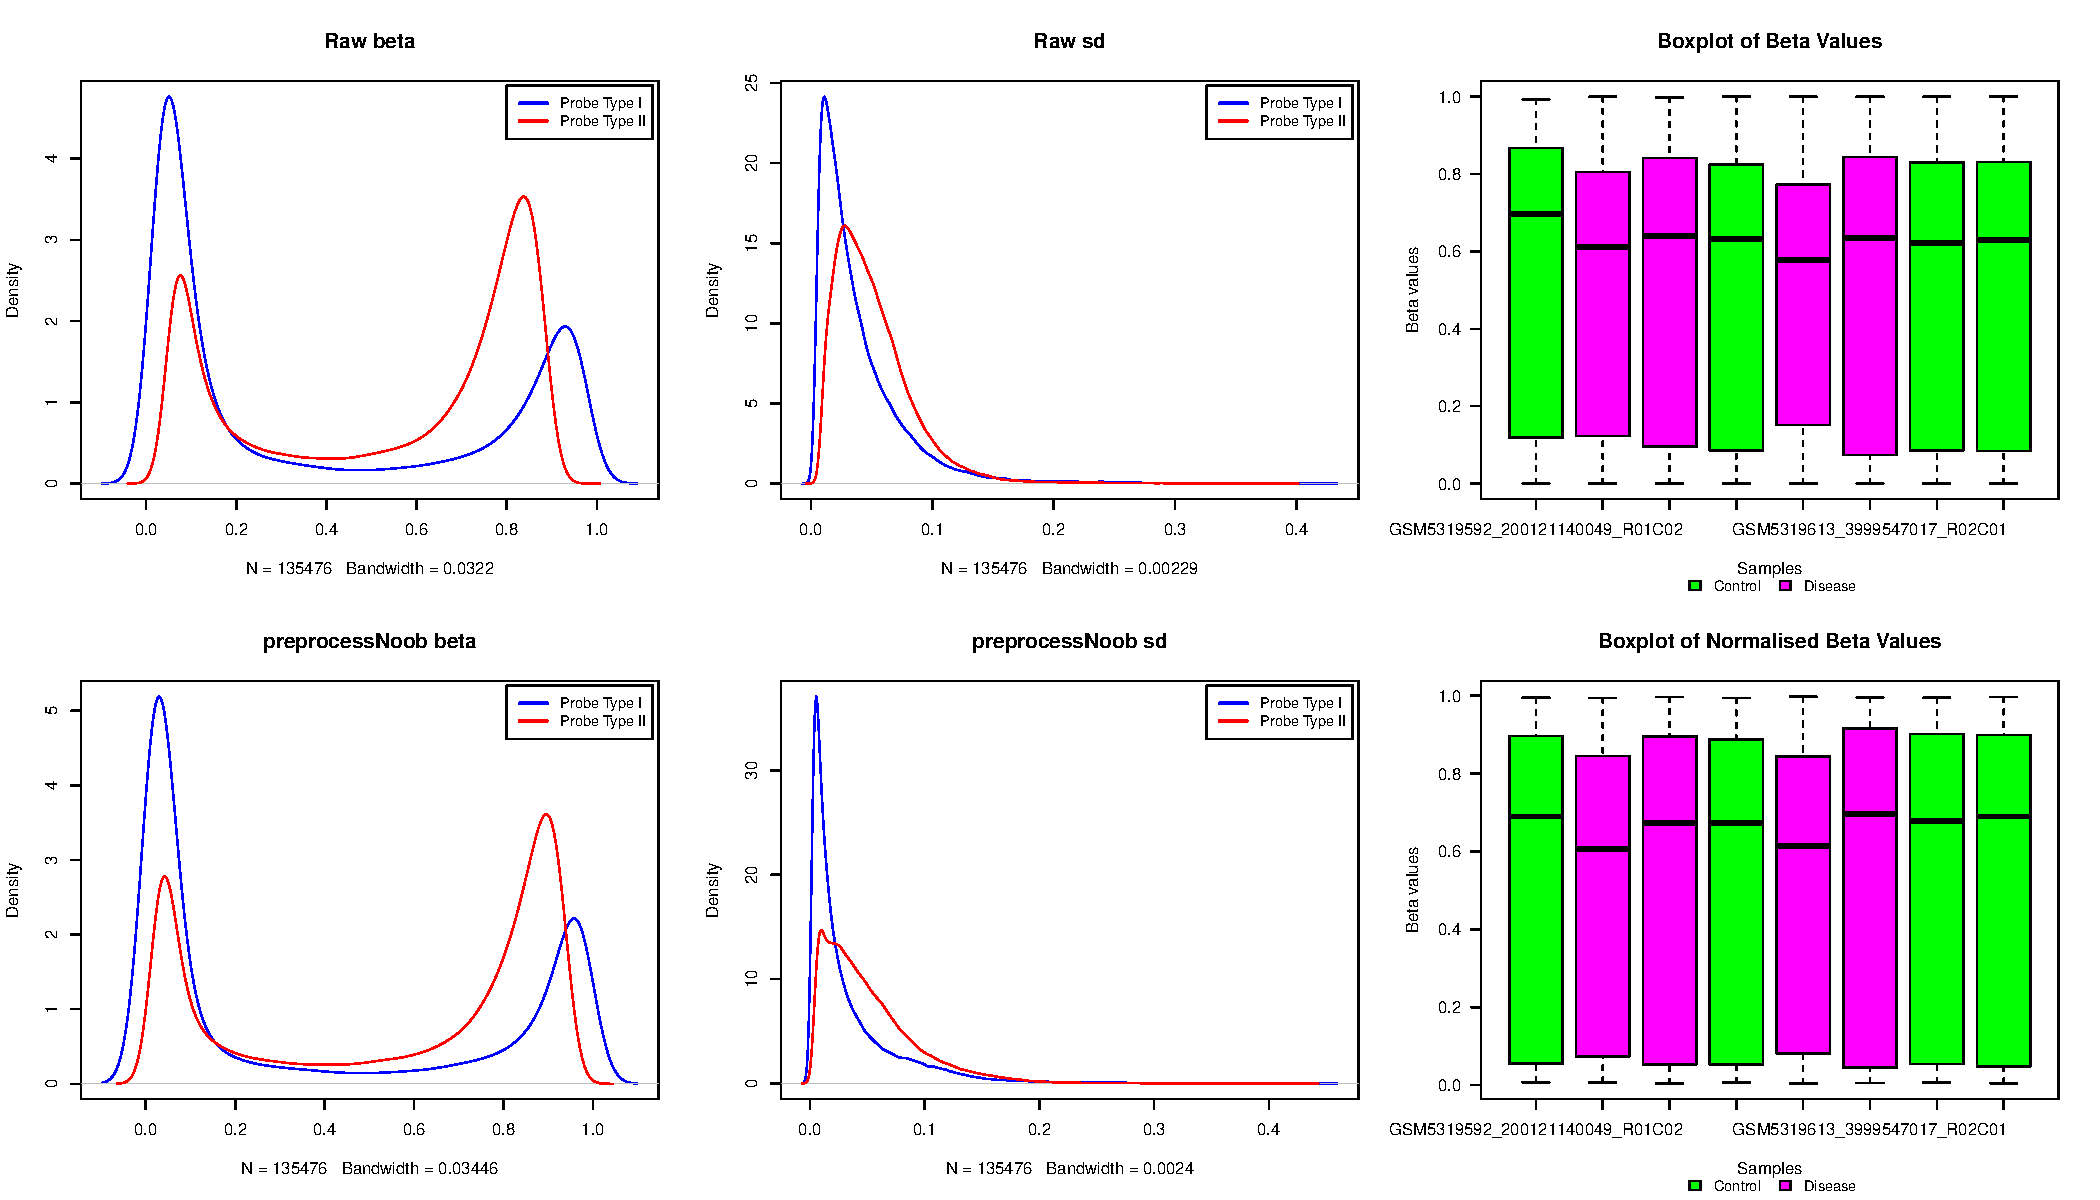
\includegraphics[keepaspectratio]{../results/BetaValuesBoxPlot-1.pdf}}

\textbf{Comment:} preprocessNoob is a normalization method designed to
correct background fluorescence and dye bias. It is known as a ``light''
normalization technique, meaning it applies minimal transformation to
the data while still addressing key technical artifacts.

After applying it, the density plots show that the probe type
distributions are slightly more aligned, indicating improved
consistency. However, the boxplots reveal a larger interquartile range
and non-uniform medians across samples, suggesting that some variability
remains uncorrected.

Given these results, preprocessNoob may not be the most appropriate
normalization method for this dataset. Although it effectively corrects
background noise and dye bias, it does not sufficiently address sample
variability. A better alternative could be preprocessQuantile, which
applies stratified quantile normalization specifically tailored for
Illumina methylation microarrays---the platform used for this dataset.

\subsection{STEP 8. Principal Component
Analysis}\label{step-8.-principal-component-analysis}

Perform a PCA on the matrix of normalized beta values generated in step
7.

\textbf{Perform PCA on normalized beta values}

\begin{Shaded}
\begin{Highlighting}[]
\NormalTok{pca\_results }\OtherTok{\textless{}{-}} \FunctionTok{prcomp}\NormalTok{(}\FunctionTok{t}\NormalTok{(beta\_preprocessNoob), }\AttributeTok{scale =} \ConstantTok{TRUE}\NormalTok{)}
\NormalTok{pca\_var }\OtherTok{\textless{}{-}}\NormalTok{ pca\_results}\SpecialCharTok{$}\NormalTok{sdev}\SpecialCharTok{\^{}}\DecValTok{2}
\NormalTok{pca\_var\_explained }\OtherTok{\textless{}{-}}\NormalTok{ pca\_var }\SpecialCharTok{/} \FunctionTok{sum}\NormalTok{(pca\_var)}
\FunctionTok{barplot}\NormalTok{(pca\_var\_explained[}\DecValTok{1}\SpecialCharTok{:}\DecValTok{10}\NormalTok{], }
        \AttributeTok{names.arg =} \FunctionTok{paste0}\NormalTok{(}\StringTok{"PC"}\NormalTok{, }\DecValTok{1}\SpecialCharTok{:}\DecValTok{10}\NormalTok{),}
        \AttributeTok{col =} \StringTok{"blue"}\NormalTok{,}
        \AttributeTok{main =} \StringTok{"Scree Plot: Variance Explained by PCs"}\NormalTok{,}
        \AttributeTok{xlab =} \StringTok{"Principal Components"}\NormalTok{,}
        \AttributeTok{ylab =} \StringTok{"Proportion of Variance Explained"}\NormalTok{,}
        \AttributeTok{las =} \DecValTok{2}\NormalTok{)}
\end{Highlighting}
\end{Shaded}

\pandocbounded{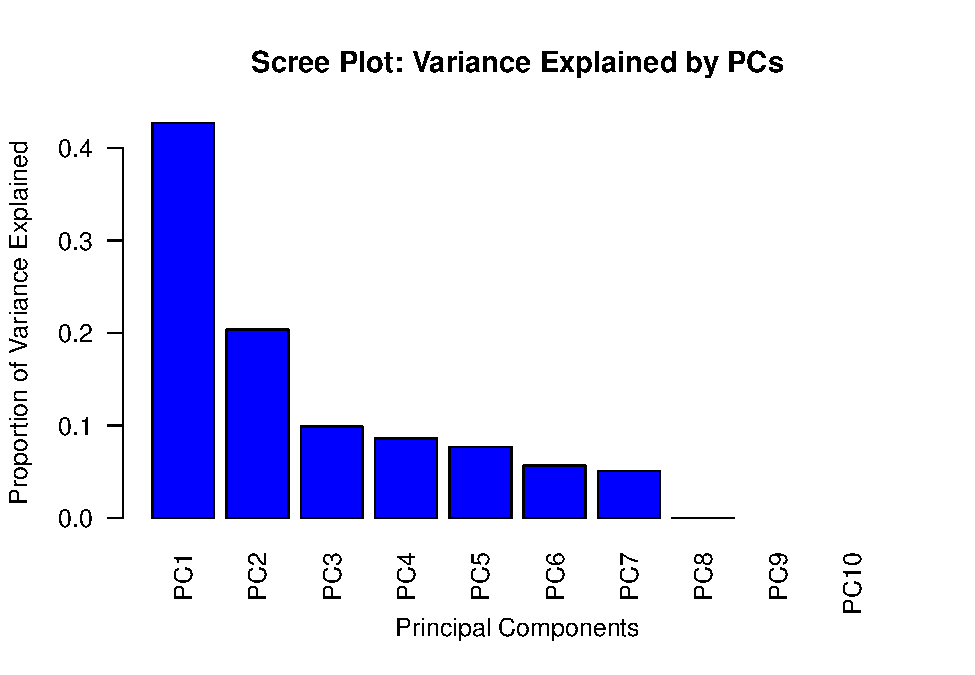
\includegraphics[keepaspectratio]{../results/ScreePlotPCA-1.pdf}}

\textbf{Plot PCA by Group}

\begin{Shaded}
\begin{Highlighting}[]
\FunctionTok{par}\NormalTok{(}\AttributeTok{mfrow =} \FunctionTok{c}\NormalTok{(}\DecValTok{1}\NormalTok{, }\DecValTok{1}\NormalTok{)) }
\FunctionTok{palette}\NormalTok{(}\FunctionTok{c}\NormalTok{(}\StringTok{\textquotesingle{}orange\textquotesingle{}}\NormalTok{, }\StringTok{\textquotesingle{}green\textquotesingle{}}\NormalTok{))}
\FunctionTok{plot}\NormalTok{(pca\_results}\SpecialCharTok{$}\NormalTok{x[, }\DecValTok{1}\NormalTok{], pca\_results}\SpecialCharTok{$}\NormalTok{x[, }\DecValTok{2}\NormalTok{], }\AttributeTok{cex =} \DecValTok{1}\NormalTok{, }\AttributeTok{pch =} \DecValTok{17}\NormalTok{, }\AttributeTok{col =}\NormalTok{ pheno}\SpecialCharTok{$}\NormalTok{Group, }
     \AttributeTok{main =} \StringTok{\textquotesingle{}PCA by group\textquotesingle{}}\NormalTok{, }\AttributeTok{xlab =} \StringTok{"PC1"}\NormalTok{, }\AttributeTok{ylab =} \StringTok{"PC2"}\NormalTok{, }\AttributeTok{xlim =} \FunctionTok{c}\NormalTok{(}\SpecialCharTok{{-}}\DecValTok{1000}\NormalTok{, }\DecValTok{1000}\NormalTok{), }\AttributeTok{ylim =} \FunctionTok{c}\NormalTok{(}\SpecialCharTok{{-}}\DecValTok{1000}\NormalTok{, }\DecValTok{1000}\NormalTok{))}
\FunctionTok{text}\NormalTok{(pca\_results}\SpecialCharTok{$}\NormalTok{x[, }\DecValTok{1}\NormalTok{], pca\_results}\SpecialCharTok{$}\NormalTok{x[, }\DecValTok{2}\NormalTok{], }\AttributeTok{labels =}\NormalTok{ (pheno}\SpecialCharTok{$}\NormalTok{SampleID), }\AttributeTok{cex =} \FloatTok{0.7}\NormalTok{, }\AttributeTok{pos =} \DecValTok{1}\NormalTok{)}
\FunctionTok{legend}\NormalTok{(}\StringTok{\textquotesingle{}bottomright\textquotesingle{}}\NormalTok{, }\AttributeTok{legend =} \FunctionTok{levels}\NormalTok{(pheno}\SpecialCharTok{$}\NormalTok{Group), }\AttributeTok{col =} \FunctionTok{c}\NormalTok{(}\DecValTok{1}\SpecialCharTok{:}\FunctionTok{nlevels}\NormalTok{(pheno}\SpecialCharTok{$}\NormalTok{Group)), }\AttributeTok{pch =} \DecValTok{17}\NormalTok{)}
\end{Highlighting}
\end{Shaded}

\pandocbounded{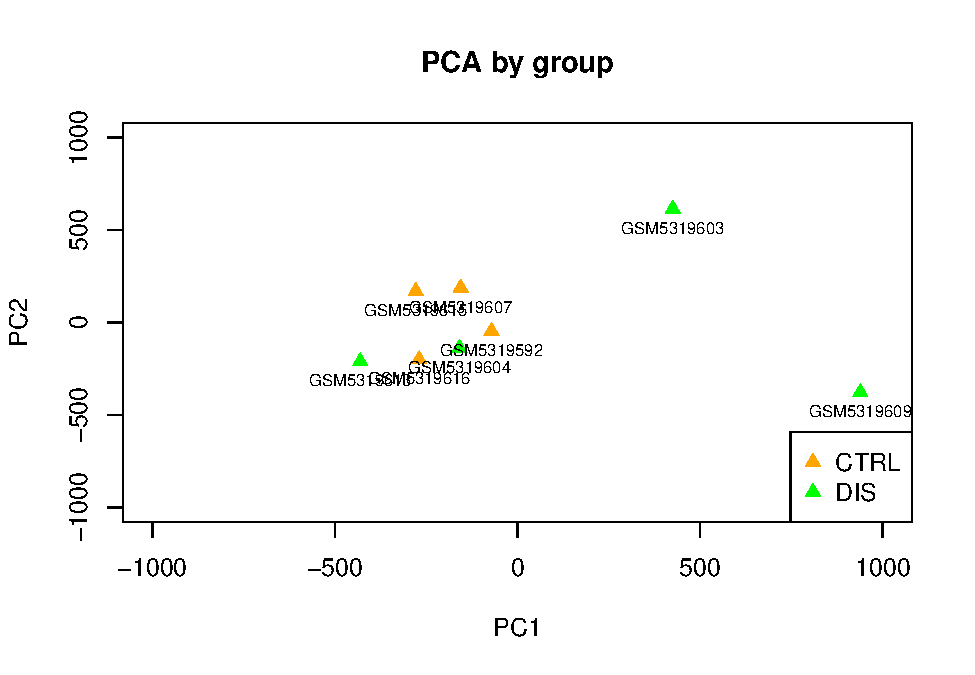
\includegraphics[keepaspectratio]{../results/GroupedPCA-1.pdf}}

\textbf{Comment:} Unfortunately, the PCA analysis does not show a clear
separation between the control and disease groups. While the control
samples cluster closely together, the disease samples are more dispersed
across the plot.

\textbf{Plot PCA by Sex}

\begin{Shaded}
\begin{Highlighting}[]
\NormalTok{pheno}\SpecialCharTok{$}\NormalTok{Sex}
\NormalTok{pheno}\SpecialCharTok{$}\NormalTok{Sex }\OtherTok{\textless{}{-}} \FunctionTok{as.factor}\NormalTok{(pheno}\SpecialCharTok{$}\NormalTok{Sex)}
\FunctionTok{palette}\NormalTok{(}\FunctionTok{c}\NormalTok{(}\StringTok{\textquotesingle{}pink\textquotesingle{}}\NormalTok{, }\StringTok{\textquotesingle{}aquamarine\textquotesingle{}}\NormalTok{))}
\FunctionTok{plot}\NormalTok{(pca\_results}\SpecialCharTok{$}\NormalTok{x[, }\DecValTok{1}\NormalTok{], pca\_results}\SpecialCharTok{$}\NormalTok{x[, }\DecValTok{2}\NormalTok{], }\AttributeTok{cex =} \DecValTok{2}\NormalTok{, }\AttributeTok{pch =} \DecValTok{17}\NormalTok{, }\AttributeTok{col =}\NormalTok{ pheno}\SpecialCharTok{$}\NormalTok{Sex, }
     \AttributeTok{main =} \StringTok{\textquotesingle{}PCA by sex\textquotesingle{}}\NormalTok{, }\AttributeTok{xlab =} \StringTok{"PC1"}\NormalTok{, }\AttributeTok{ylab =} \StringTok{"PC2"}\NormalTok{, }\AttributeTok{xlim =} \FunctionTok{c}\NormalTok{(}\SpecialCharTok{{-}}\DecValTok{1000}\NormalTok{, }\DecValTok{1000}\NormalTok{), }\AttributeTok{ylim =} \FunctionTok{c}\NormalTok{(}\SpecialCharTok{{-}}\DecValTok{1000}\NormalTok{, }\DecValTok{1000}\NormalTok{))}
\FunctionTok{text}\NormalTok{(pca\_results}\SpecialCharTok{$}\NormalTok{x[, }\DecValTok{1}\NormalTok{], pca\_results}\SpecialCharTok{$}\NormalTok{x[, }\DecValTok{2}\NormalTok{], }\AttributeTok{labels =}\NormalTok{ (pheno}\SpecialCharTok{$}\NormalTok{SampleID), }\AttributeTok{cex =} \FloatTok{0.7}\NormalTok{, }\AttributeTok{pos =} \DecValTok{1}\NormalTok{)}
\FunctionTok{legend}\NormalTok{(}\StringTok{\textquotesingle{}bottomright\textquotesingle{}}\NormalTok{, }\AttributeTok{legend =} \FunctionTok{levels}\NormalTok{(pheno}\SpecialCharTok{$}\NormalTok{Sex), }\AttributeTok{col =} \FunctionTok{c}\NormalTok{(}\DecValTok{1}\SpecialCharTok{:}\FunctionTok{nlevels}\NormalTok{(pheno}\SpecialCharTok{$}\NormalTok{Sex)), }\AttributeTok{pch =} \DecValTok{17}\NormalTok{)}
\end{Highlighting}
\end{Shaded}

\pandocbounded{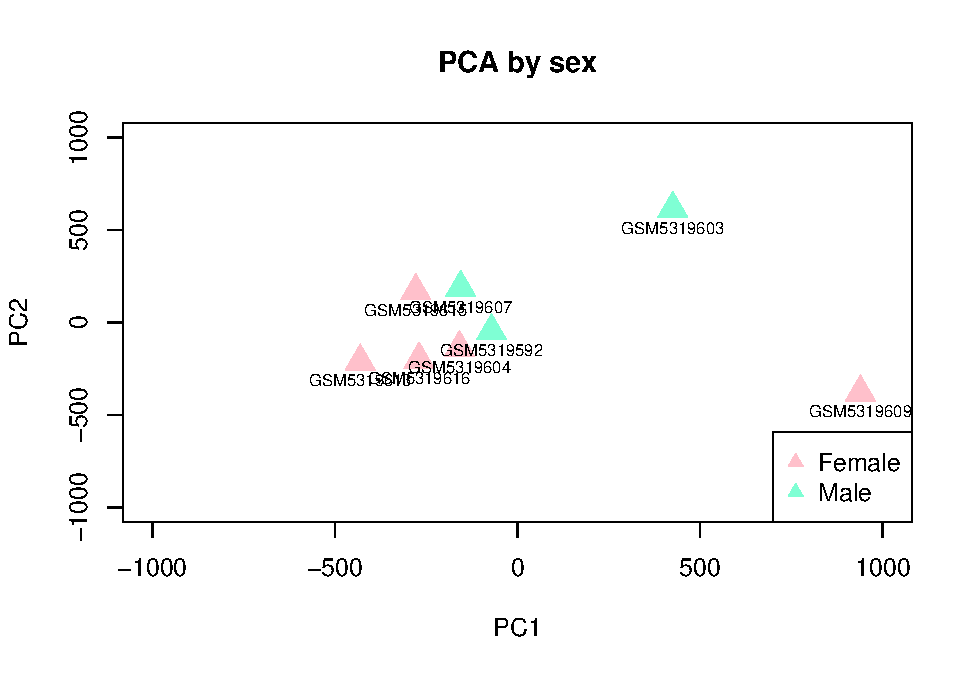
\includegraphics[keepaspectratio]{../results/SexPCA-1.pdf}}

\textbf{Comment:} In this PCA analysis, the female samples cluster
closely together, with the exception of one outlier (GMS5319609), but
there is not a clear separation based on sex.

\textbf{Plot PCA by Sentrix\_ID}

\begin{Shaded}
\begin{Highlighting}[]
\NormalTok{pheno}\SpecialCharTok{$}\NormalTok{Sentrix\_ID}
\NormalTok{pheno}\SpecialCharTok{$}\NormalTok{Sentrix\_ID }\OtherTok{\textless{}{-}} \FunctionTok{as.factor}\NormalTok{(pheno}\SpecialCharTok{$}\NormalTok{Sentrix\_ID)}
\FunctionTok{palette}\NormalTok{(}\FunctionTok{c}\NormalTok{(}\StringTok{\textquotesingle{}red\textquotesingle{}}\NormalTok{, }\StringTok{\textquotesingle{}blue\textquotesingle{}}\NormalTok{, }\StringTok{\textquotesingle{}green\textquotesingle{}}\NormalTok{, }\StringTok{\textquotesingle{}yellow\textquotesingle{}}\NormalTok{, }\StringTok{\textquotesingle{}purple\textquotesingle{}}\NormalTok{))}
\FunctionTok{plot}\NormalTok{(pca\_results}\SpecialCharTok{$}\NormalTok{x[, }\DecValTok{1}\NormalTok{], pca\_results}\SpecialCharTok{$}\NormalTok{x[, }\DecValTok{2}\NormalTok{], }\AttributeTok{cex =} \DecValTok{2}\NormalTok{, }\AttributeTok{pch =} \DecValTok{17}\NormalTok{, }\AttributeTok{col =}\NormalTok{ pheno}\SpecialCharTok{$}\NormalTok{Sentrix\_ID, }
     \AttributeTok{main =} \StringTok{\textquotesingle{}PCA by Sentrix\_ID\textquotesingle{}}\NormalTok{, }\AttributeTok{xlab =} \StringTok{"PC1"}\NormalTok{, }\AttributeTok{ylab =} \StringTok{"PC2"}\NormalTok{, }\AttributeTok{xlim =} \FunctionTok{c}\NormalTok{(}\SpecialCharTok{{-}}\DecValTok{1000}\NormalTok{, }\DecValTok{1000}\NormalTok{), }
     \AttributeTok{ylim =} \FunctionTok{c}\NormalTok{(}\SpecialCharTok{{-}}\DecValTok{1000}\NormalTok{, }\DecValTok{1000}\NormalTok{))}
\FunctionTok{text}\NormalTok{(pca\_results}\SpecialCharTok{$}\NormalTok{x[, }\DecValTok{1}\NormalTok{], pca\_results}\SpecialCharTok{$}\NormalTok{x[, }\DecValTok{2}\NormalTok{], }\AttributeTok{labels =}\NormalTok{ (pheno}\SpecialCharTok{$}\NormalTok{SampleID), }\AttributeTok{cex =} \FloatTok{0.7}\NormalTok{, }\AttributeTok{pos =} \DecValTok{1}\NormalTok{)}
\FunctionTok{legend}\NormalTok{(}\StringTok{\textquotesingle{}topleft\textquotesingle{}}\NormalTok{, }\AttributeTok{legend =} \FunctionTok{levels}\NormalTok{(pheno}\SpecialCharTok{$}\NormalTok{Sentrix\_ID), }
       \AttributeTok{col =} \FunctionTok{c}\NormalTok{(}\DecValTok{1}\SpecialCharTok{:}\FunctionTok{nlevels}\NormalTok{(pheno}\SpecialCharTok{$}\NormalTok{Sentrix\_ID)), }\AttributeTok{pch =} \DecValTok{17}\NormalTok{)}
\end{Highlighting}
\end{Shaded}

\pandocbounded{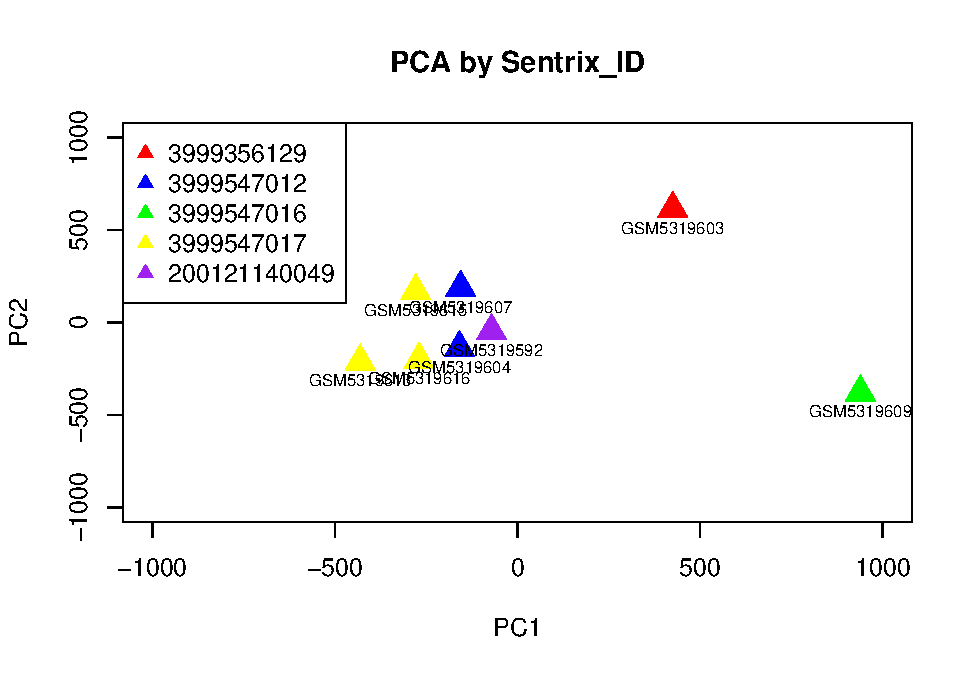
\includegraphics[keepaspectratio]{../results/SentrixIdPCA-1.pdf}}

\textbf{Comment:} Five batches were identified. The PCA shows
clustering; however, there are almost as many batches as there are
samples. This makes it difficult to determine whether the variability
observed in the experimental results is due to batch effects. A larger
sample size would be needed to confirm this.

\subsection{STEP 9. Differential Methylation
Analysis}\label{step-9.-differential-methylation-analysis}

Using the matrix of normalized beta values generated in step 7, identify
differentially methylated probes between CTRL and DIS groups using a
t-test.

\textbf{Example for a single probe}

\begin{Shaded}
\begin{Highlighting}[]
\NormalTok{t\_test }\OtherTok{\textless{}{-}} \FunctionTok{t.test}\NormalTok{(beta\_preprocessNoob[}\DecValTok{1}\NormalTok{, ] }\SpecialCharTok{\textasciitilde{}}\NormalTok{ pheno}\SpecialCharTok{$}\NormalTok{Group)}
\NormalTok{t\_test}
\NormalTok{t\_test}\SpecialCharTok{$}\NormalTok{p.value}
\end{Highlighting}
\end{Shaded}

\textbf{Define a function to apply test to all probes}

\begin{Shaded}
\begin{Highlighting}[]
\NormalTok{My\_ttest\_function }\OtherTok{\textless{}{-}} \ControlFlowTok{function}\NormalTok{(x) \{}
\NormalTok{  t\_test }\OtherTok{\textless{}{-}} \FunctionTok{t.test}\NormalTok{(x }\SpecialCharTok{\textasciitilde{}}\NormalTok{ pheno}\SpecialCharTok{$}\NormalTok{Group)}
  \FunctionTok{return}\NormalTok{(t\_test}\SpecialCharTok{$}\NormalTok{p.value)}
\NormalTok{\}}
\end{Highlighting}
\end{Shaded}

\textbf{Apply the function to all probes}

\begin{Shaded}
\begin{Highlighting}[]
\NormalTok{pValues\_ttest }\OtherTok{\textless{}{-}} \FunctionTok{apply}\NormalTok{(beta\_preprocessNoob, }\DecValTok{1}\NormalTok{, My\_ttest\_function)}
\end{Highlighting}
\end{Shaded}

\textbf{Create data.frame with beta values and p-values}

\begin{Shaded}
\begin{Highlighting}[]
\NormalTok{final\_ttest }\OtherTok{\textless{}{-}} \FunctionTok{data.frame}\NormalTok{(beta\_preprocessNoob, pValues\_ttest)}
\end{Highlighting}
\end{Shaded}

\textbf{Order probes by p-value}

\begin{Shaded}
\begin{Highlighting}[]
\NormalTok{final\_ttest }\OtherTok{\textless{}{-}}\NormalTok{ final\_ttest[}\FunctionTok{order}\NormalTok{(final\_ttest}\SpecialCharTok{$}\NormalTok{pValues\_ttest), ]}
\FunctionTok{head}\NormalTok{(final\_ttest)}
\end{Highlighting}
\end{Shaded}

\textbf{Filter for significant probes (p \textless{} 0.05)}

\begin{Shaded}
\begin{Highlighting}[]
\NormalTok{significant\_ttest }\OtherTok{\textless{}{-}}\NormalTok{ final\_ttest[final\_ttest}\SpecialCharTok{$}\NormalTok{pValues\_ttest }\SpecialCharTok{\textless{}=} \FloatTok{0.05}\NormalTok{, ]}
\end{Highlighting}
\end{Shaded}

\subsection{STEP 10. Multiple Test
Correction}\label{step-10.-multiple-test-correction}

\textbf{Apply multiple test correction and set a significant threshold
of 0.05}

\begin{Shaded}
\begin{Highlighting}[]
\NormalTok{corrected\_pValues\_BH }\OtherTok{\textless{}{-}} \FunctionTok{p.adjust}\NormalTok{(final\_ttest}\SpecialCharTok{$}\NormalTok{pValues\_ttest, }\StringTok{"BH"}\NormalTok{)}
\NormalTok{corrected\_pValues\_Bonf }\OtherTok{\textless{}{-}} \FunctionTok{p.adjust}\NormalTok{(final\_ttest}\SpecialCharTok{$}\NormalTok{pValues\_ttest, }\StringTok{"bonferroni"}\NormalTok{)}
\NormalTok{final\_ttest\_corrected }\OtherTok{\textless{}{-}} \FunctionTok{data.frame}\NormalTok{(final\_ttest, corrected\_pValues\_BH, corrected\_pValues\_Bonf)}
\FunctionTok{head}\NormalTok{(final\_ttest\_corrected)}
\end{Highlighting}
\end{Shaded}

\textbf{Visualize distributions of p-values and corrected p-values}

\begin{Shaded}
\begin{Highlighting}[]
\FunctionTok{colnames}\NormalTok{(final\_ttest\_corrected)}
\NormalTok{box\_colors }\OtherTok{\textless{}{-}} \FunctionTok{c}\NormalTok{(}\StringTok{"skyblue"}\NormalTok{, }\StringTok{"lightgreen"}\NormalTok{, }\StringTok{"salmon"}\NormalTok{)}
\FunctionTok{boxplot}\NormalTok{(final\_ttest\_corrected[, }\DecValTok{9}\SpecialCharTok{:}\DecValTok{11}\NormalTok{],}
        \AttributeTok{main =} \StringTok{"Distribution of Raw and Corrected p{-}values"}\NormalTok{,}
        \AttributeTok{ylab =} \StringTok{"p{-}values"}\NormalTok{,}
        \AttributeTok{xlab =} \StringTok{"Correction Method"}\NormalTok{,}
        \AttributeTok{col =}\NormalTok{ box\_colors,}
        \AttributeTok{names =} \FunctionTok{c}\NormalTok{(}\StringTok{"Raw"}\NormalTok{, }\StringTok{"BH"}\NormalTok{, }\StringTok{"Bonferroni"}\NormalTok{))}
\FunctionTok{legend}\NormalTok{(}\StringTok{"bottomright"}\NormalTok{,}
       \AttributeTok{legend =} \FunctionTok{c}\NormalTok{(}\StringTok{"Raw"}\NormalTok{, }\StringTok{"BH"}\NormalTok{, }\StringTok{"Bonferroni"}\NormalTok{),}
       \AttributeTok{fill =}\NormalTok{ box\_colors,}
       \AttributeTok{cex =} \FloatTok{0.8}\NormalTok{)}
\end{Highlighting}
\end{Shaded}

\pandocbounded{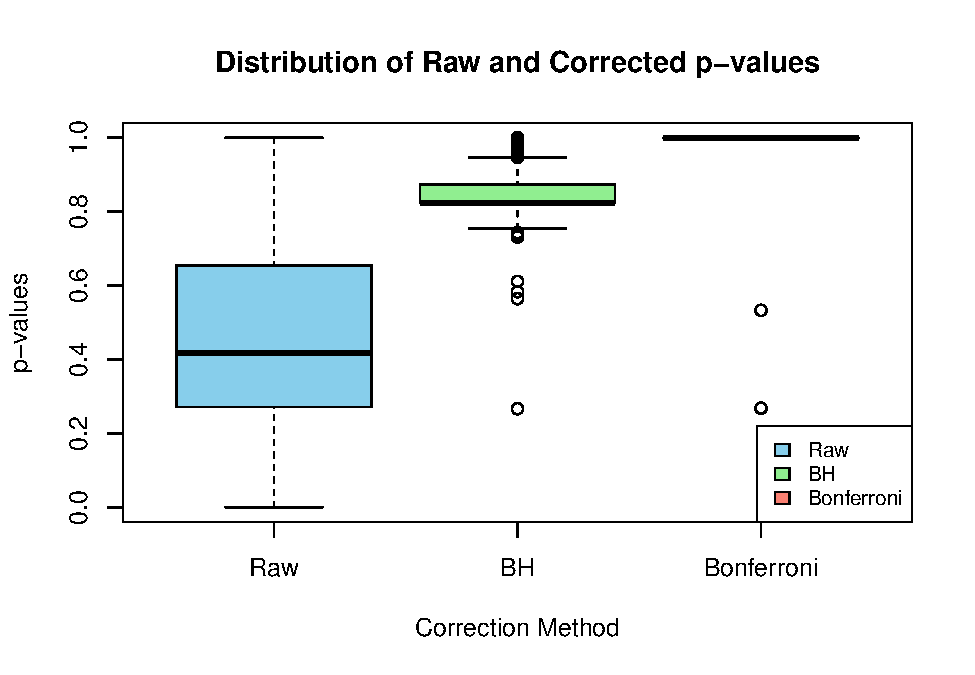
\includegraphics[keepaspectratio]{../results/PvalDistributions-1.pdf}}

\textbf{Determining the amount of probes that remain after the MTC}

\begin{Shaded}
\begin{Highlighting}[]
\FunctionTok{dim}\NormalTok{(final\_ttest\_corrected[final\_ttest\_corrected}\SpecialCharTok{$}\NormalTok{pValues\_ttest }\SpecialCharTok{\textless{}=} \FloatTok{0.05}\NormalTok{, ])}
\FunctionTok{dim}\NormalTok{(final\_ttest\_corrected[final\_ttest\_corrected}\SpecialCharTok{$}\NormalTok{corrected\_pValues\_BH }\SpecialCharTok{\textless{}=} \FloatTok{0.05}\NormalTok{, ])}
\FunctionTok{dim}\NormalTok{(final\_ttest\_corrected[final\_ttest\_corrected}\SpecialCharTok{$}\NormalTok{corrected\_pValues\_Bonf }\SpecialCharTok{\textless{}=} \FloatTok{0.05}\NormalTok{, ])}
\end{Highlighting}
\end{Shaded}

\textbf{Comment:} 11,928 probes with a nominal p-value below 0.05 before
applying any multiple testing correction were identified. However, after
applying Bonferroni and Benjamini-Hochberg (BH) corrections, no probes
remained significant at the 0.05 threshold. This suggests that while
many probes appeared significant before correction, these results may be
due to chance, highlighting the importance of correcting for multiple
testing in high-dimensional data like DNA methylation. Furthermore, this
could also be an additional sign that the normalization procedure
applied to data was not appropriate. Most likely, applying the
preprocessQuantile function and then the t-test on data, the multiple
testing correction may highlight significant probes.

\subsection{STEP 11. Graphic the results of the differential methylation
analysis.}\label{step-11.-graphic-the-results-of-the-differential-methylation-analysis.}

Produce a volcano plot and a Manhattan plot of the results of
differential methylation analysis.

\textbf{a. Volcano plot}

Preparation of the data

\begin{Shaded}
\begin{Highlighting}[]
\NormalTok{beta\_first }\OtherTok{\textless{}{-}}\NormalTok{ final\_ttest\_corrected[, }\DecValTok{1}\SpecialCharTok{:}\DecValTok{8}\NormalTok{]}
\NormalTok{beta\_first\_ctrl }\OtherTok{\textless{}{-}}\NormalTok{ beta\_first[, pheno}\SpecialCharTok{$}\NormalTok{Group }\SpecialCharTok{==} \StringTok{"CTRL"}\NormalTok{]}
\NormalTok{beta\_first\_dis }\OtherTok{\textless{}{-}}\NormalTok{ beta\_first[, pheno}\SpecialCharTok{$}\NormalTok{Group }\SpecialCharTok{==} \StringTok{"DIS"}\NormalTok{]}
\NormalTok{mean\_beta\_first\_ctrl }\OtherTok{\textless{}{-}} \FunctionTok{apply}\NormalTok{(beta\_first\_ctrl, }\DecValTok{1}\NormalTok{, mean)}
\NormalTok{mean\_beta\_first\_dis }\OtherTok{\textless{}{-}} \FunctionTok{apply}\NormalTok{(beta\_first\_dis, }\DecValTok{1}\NormalTok{, mean)}
\NormalTok{delta\_first }\OtherTok{\textless{}{-}}\NormalTok{ mean\_beta\_first\_dis }\SpecialCharTok{{-}}\NormalTok{ mean\_beta\_first\_ctrl}
\NormalTok{toVolcPlot }\OtherTok{\textless{}{-}} \FunctionTok{data.frame}\NormalTok{(}
  \AttributeTok{delta\_beta =}\NormalTok{ delta\_first,}
  \AttributeTok{negLog10p =} \SpecialCharTok{{-}}\FunctionTok{log10}\NormalTok{(final\_ttest\_corrected}\SpecialCharTok{$}\NormalTok{pValues\_ttest)}
\NormalTok{)}
\end{Highlighting}
\end{Shaded}

Volcano plot to highlight hypermethylated (Delta Beta \textgreater{} 0.1
\& p \textless{} 0.05) and hypomethylated (Delta Beta \textless{} -0.1
\& p \textless{} 0.05) targets

\begin{Shaded}
\begin{Highlighting}[]
\FunctionTok{plot}\NormalTok{(toVolcPlot}\SpecialCharTok{$}\NormalTok{delta\_beta, toVolcPlot}\SpecialCharTok{$}\NormalTok{negLog10p,}
     \AttributeTok{pch =} \DecValTok{16}\NormalTok{, }\AttributeTok{cex =} \FloatTok{0.5}\NormalTok{,}
     \AttributeTok{xlab =} \StringTok{"Delta Beta (DIS {-} CTRL)"}\NormalTok{,}
     \AttributeTok{ylab =} \StringTok{"{-}log10(p{-}value)"}\NormalTok{,}
     \AttributeTok{main =} \StringTok{"Volcano Plot of Methylation Differences"}\NormalTok{)}
\NormalTok{hyper }\OtherTok{\textless{}{-}} \FunctionTok{which}\NormalTok{(toVolcPlot}\SpecialCharTok{$}\NormalTok{delta\_beta }\SpecialCharTok{\textgreater{}} \FloatTok{0.1} \SpecialCharTok{\&}\NormalTok{ final\_ttest\_corrected}\SpecialCharTok{$}\NormalTok{pValues\_ttest }\SpecialCharTok{\textless{}} \FloatTok{0.05}\NormalTok{)}
\FunctionTok{points}\NormalTok{(toVolcPlot}\SpecialCharTok{$}\NormalTok{delta\_beta[hyper],}
\NormalTok{       toVolcPlot}\SpecialCharTok{$}\NormalTok{negLog10p[hyper],}
       \AttributeTok{col =} \StringTok{"red"}\NormalTok{, }\AttributeTok{pch =} \DecValTok{16}\NormalTok{, }\AttributeTok{cex =} \FloatTok{0.6}\NormalTok{)}
\NormalTok{hypo }\OtherTok{\textless{}{-}} \FunctionTok{which}\NormalTok{(toVolcPlot}\SpecialCharTok{$}\NormalTok{delta\_beta }\SpecialCharTok{\textless{}} \SpecialCharTok{{-}}\FloatTok{0.1} \SpecialCharTok{\&}\NormalTok{ final\_ttest\_corrected}\SpecialCharTok{$}\NormalTok{pValues\_ttest }\SpecialCharTok{\textless{}} \FloatTok{0.05}\NormalTok{)}
\FunctionTok{points}\NormalTok{(toVolcPlot}\SpecialCharTok{$}\NormalTok{delta\_beta[hypo],}
\NormalTok{       toVolcPlot}\SpecialCharTok{$}\NormalTok{negLog10p[hypo],}
       \AttributeTok{col =} \StringTok{"blue"}\NormalTok{, }\AttributeTok{pch =} \DecValTok{16}\NormalTok{, }\AttributeTok{cex =} \FloatTok{0.6}\NormalTok{)}

\FunctionTok{abline}\NormalTok{(}\AttributeTok{h =} \SpecialCharTok{{-}}\FunctionTok{log10}\NormalTok{(}\FloatTok{0.05}\NormalTok{), }\AttributeTok{col =} \StringTok{"darkgray"}\NormalTok{, }\AttributeTok{lty =} \DecValTok{2}\NormalTok{)  }\CommentTok{\# p = 0.05}
\FunctionTok{abline}\NormalTok{(}\AttributeTok{v =} \FunctionTok{c}\NormalTok{(}\SpecialCharTok{{-}}\FloatTok{0.1}\NormalTok{, }\FloatTok{0.1}\NormalTok{), }\AttributeTok{col =} \StringTok{"darkgray"}\NormalTok{, }\AttributeTok{lty =} \DecValTok{2}\NormalTok{)  }\CommentTok{\# Delta Beta = ±0.1}
\FunctionTok{legend}\NormalTok{(}\StringTok{"topright"}\NormalTok{, }\AttributeTok{legend =} \FunctionTok{c}\NormalTok{(}\StringTok{"Hypermethylated"}\NormalTok{, }\StringTok{"Hypomethylated"}\NormalTok{),}
       \AttributeTok{col =} \FunctionTok{c}\NormalTok{(}\StringTok{"red"}\NormalTok{, }\StringTok{"blue"}\NormalTok{), }\AttributeTok{pch =} \DecValTok{16}\NormalTok{, }\AttributeTok{bty =} \StringTok{"n"}\NormalTok{)}
\end{Highlighting}
\end{Shaded}

\pandocbounded{\includegraphics[keepaspectratio]{../results/VolcanoPlot-1.pdf}}

\textbf{b. Manhattan plot}

Annotate dataframe with genome annotation for each CpG probe.

\begin{Shaded}
\begin{Highlighting}[]
\NormalTok{final\_ttest\_corrected }\OtherTok{\textless{}{-}} \FunctionTok{data.frame}\NormalTok{(}\FunctionTok{rownames}\NormalTok{(final\_ttest\_corrected), final\_ttest\_corrected)}
\FunctionTok{colnames}\NormalTok{(final\_ttest\_corrected)[}\DecValTok{1}\NormalTok{] }\OtherTok{\textless{}{-}} \StringTok{"IlmnID"}
\NormalTok{final\_ttest\_corrected\_clean }\OtherTok{\textless{}{-}}\NormalTok{ final\_ttest\_corrected[, }\SpecialCharTok{!}\FunctionTok{duplicated}\NormalTok{(}\FunctionTok{colnames}\NormalTok{(final\_ttest\_corrected))]}
\NormalTok{final\_ttest\_corrected\_annotated }\OtherTok{\textless{}{-}} \FunctionTok{merge}\NormalTok{(final\_ttest\_corrected\_clean, Illumina450Manifest\_clean, }
                                   \AttributeTok{by =} \StringTok{"IlmnID"}\NormalTok{)}
\NormalTok{input\_Manhattan }\OtherTok{\textless{}{-}}\NormalTok{ final\_ttest\_corrected\_annotated[}\FunctionTok{colnames}\NormalTok{(final\_ttest\_corrected\_annotated) }\SpecialCharTok{\%in\%} 
                    \FunctionTok{c}\NormalTok{(}\StringTok{"IlmnID"}\NormalTok{, }\StringTok{"CHR"}\NormalTok{, }\StringTok{"MAPINFO"}\NormalTok{, }\StringTok{"pValues\_ttest"}\NormalTok{)]}
\NormalTok{order\_chr }\OtherTok{\textless{}{-}} \FunctionTok{c}\NormalTok{(}\StringTok{"1"}\NormalTok{, }\StringTok{"2"}\NormalTok{, }\StringTok{"3"}\NormalTok{, }\StringTok{"4"}\NormalTok{, }\StringTok{"5"}\NormalTok{, }\StringTok{"6"}\NormalTok{, }\StringTok{"7"}\NormalTok{, }\StringTok{"8"}\NormalTok{, }\StringTok{"9"}\NormalTok{, }\StringTok{"10"}\NormalTok{, }\StringTok{"11"}\NormalTok{, }\StringTok{"12"}\NormalTok{, }\StringTok{"13"}\NormalTok{, }\StringTok{"14"}\NormalTok{, }\StringTok{"15"}\NormalTok{, }
               \StringTok{"16"}\NormalTok{, }\StringTok{"17"}\NormalTok{, }\StringTok{"18"}\NormalTok{, }\StringTok{"19"}\NormalTok{, }\StringTok{"20"}\NormalTok{, }\StringTok{"21"}\NormalTok{, }\StringTok{"22"}\NormalTok{, }\StringTok{"X"}\NormalTok{, }\StringTok{"Y"}\NormalTok{)}
\NormalTok{input\_Manhattan}\SpecialCharTok{$}\NormalTok{CHR }\OtherTok{\textless{}{-}} \FunctionTok{factor}\NormalTok{(input\_Manhattan}\SpecialCharTok{$}\NormalTok{CHR, }\AttributeTok{levels =}\NormalTok{ order\_chr)}
\NormalTok{input\_Manhattan}\SpecialCharTok{$}\NormalTok{CHR }\OtherTok{\textless{}{-}} \FunctionTok{as.numeric}\NormalTok{(input\_Manhattan}\SpecialCharTok{$}\NormalTok{CHR)}
\FunctionTok{manhattan}\NormalTok{(input\_Manhattan, }
          \AttributeTok{snp =} \StringTok{"IlmnID"}\NormalTok{, }
          \AttributeTok{chr =} \StringTok{"CHR"}\NormalTok{, }
          \AttributeTok{bp =} \StringTok{"MAPINFO"}\NormalTok{, }
          \AttributeTok{p =} \StringTok{"pValues\_ttest"}\NormalTok{, }
          \AttributeTok{annotatePval =} \FloatTok{0.00001}\NormalTok{, }
          \AttributeTok{col =} \FunctionTok{rainbow}\NormalTok{(}\DecValTok{24}\NormalTok{))}
\end{Highlighting}
\end{Shaded}

\pandocbounded{\includegraphics[keepaspectratio]{../results/ManhattanPlot-1.pdf}}

\subsection{STEP 12. Heatmap}\label{step-12.-heatmap}

Produce an heatmap of the top 100 significant, differentially methylated
probes.

\textbf{Define colorbar from phenotype group and custom color palette}

\begin{Shaded}
\begin{Highlighting}[]
\NormalTok{colorbar }\OtherTok{\textless{}{-}}\NormalTok{ pheno}\SpecialCharTok{$}\NormalTok{Group}
\NormalTok{colorbar }\OtherTok{\textless{}{-}} \FunctionTok{as.character}\NormalTok{(}\FunctionTok{factor}\NormalTok{(colorbar, }\AttributeTok{labels =} \FunctionTok{c}\NormalTok{(}\StringTok{"royalblue"}\NormalTok{, }\StringTok{"orange"}\NormalTok{)))}
\NormalTok{input\_heatmap }\OtherTok{=} \FunctionTok{as.matrix}\NormalTok{(final\_ttest[}\DecValTok{1}\SpecialCharTok{:}\DecValTok{100}\NormalTok{, }\DecValTok{1}\SpecialCharTok{:}\DecValTok{8}\NormalTok{])}
\NormalTok{col2 }\OtherTok{=} \FunctionTok{colorRampPalette}\NormalTok{(}\FunctionTok{c}\NormalTok{(}\StringTok{"green"}\NormalTok{, }\StringTok{"black"}\NormalTok{, }\StringTok{"red"}\NormalTok{))(}\DecValTok{100}\NormalTok{)}
\end{Highlighting}
\end{Shaded}

\textbf{Complete linkage}

\begin{Shaded}
\begin{Highlighting}[]
\FunctionTok{heatmap.2}\NormalTok{(input\_heatmap,}
          \AttributeTok{col =}\NormalTok{ col2,}
          \AttributeTok{Rowv =} \ConstantTok{TRUE}\NormalTok{,}
          \AttributeTok{Colv =} \ConstantTok{TRUE}\NormalTok{,}
          \AttributeTok{dendrogram =} \StringTok{"both"}\NormalTok{,}
          \AttributeTok{key =} \ConstantTok{TRUE}\NormalTok{,}
          \AttributeTok{ColSideColors =}\NormalTok{ colorbar,}
          \AttributeTok{density.info =} \StringTok{"none"}\NormalTok{,}
          \AttributeTok{trace =} \StringTok{"none"}\NormalTok{,}
          \AttributeTok{scale =} \StringTok{"none"}\NormalTok{,}
          \AttributeTok{symm =} \ConstantTok{FALSE}\NormalTok{,}
          \AttributeTok{main =} \StringTok{"Complete Linkage"}\NormalTok{)}
\FunctionTok{legend}\NormalTok{(}\StringTok{"topright"}\NormalTok{, }\AttributeTok{legend =} \FunctionTok{c}\NormalTok{(}\StringTok{"CTRL"}\NormalTok{, }\StringTok{"DIS"}\NormalTok{), }\AttributeTok{fill =} \FunctionTok{c}\NormalTok{(}\StringTok{"royalblue"}\NormalTok{, }\StringTok{"orange"}\NormalTok{), }\AttributeTok{border =} \ConstantTok{NA}\NormalTok{, }\AttributeTok{bty =} \StringTok{"n"}\NormalTok{, }
       \AttributeTok{cex =} \FloatTok{0.8}\NormalTok{, }\AttributeTok{xpd =} \ConstantTok{TRUE}\NormalTok{, }\AttributeTok{inset =} \FunctionTok{c}\NormalTok{(}\DecValTok{0}\NormalTok{, }\SpecialCharTok{{-}}\FloatTok{0.10}\NormalTok{))}
\end{Highlighting}
\end{Shaded}

\pandocbounded{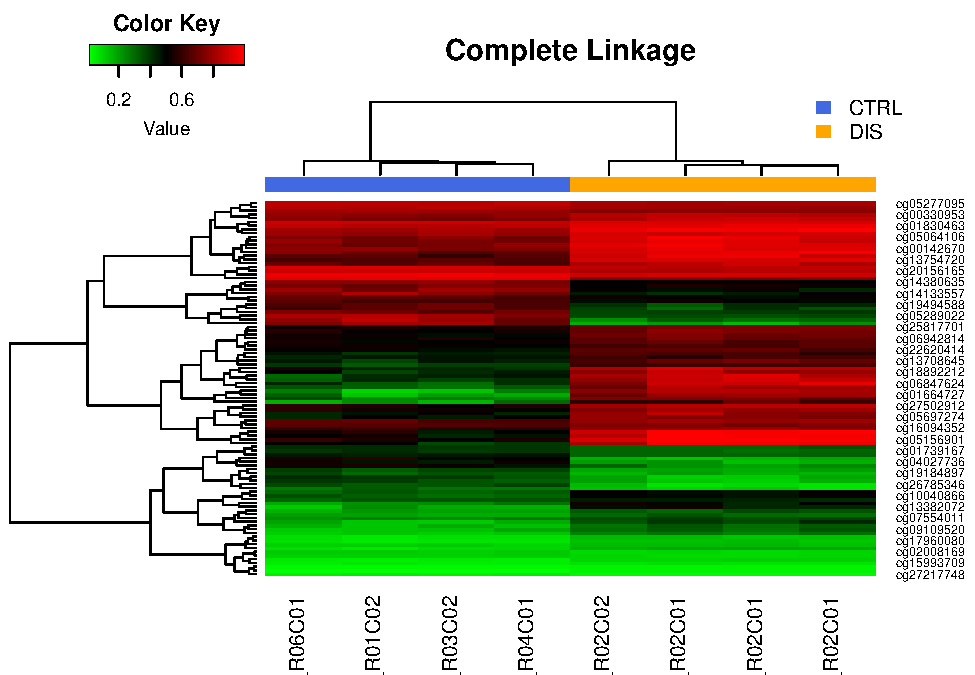
\includegraphics[keepaspectratio]{../results/HeatmapCopleteLinkage-1.pdf}}

\textbf{Single linkage}

\begin{Shaded}
\begin{Highlighting}[]
\FunctionTok{heatmap.2}\NormalTok{(input\_heatmap,}
          \AttributeTok{col =}\NormalTok{ col2,}
          \AttributeTok{Rowv =} \ConstantTok{TRUE}\NormalTok{,}
          \AttributeTok{Colv =} \ConstantTok{TRUE}\NormalTok{,}
          \AttributeTok{hclustfun =} \ControlFlowTok{function}\NormalTok{(x) }\FunctionTok{hclust}\NormalTok{(x, }\AttributeTok{method =} \StringTok{"single"}\NormalTok{),}
          \AttributeTok{dendrogram =} \StringTok{"both"}\NormalTok{,}
          \AttributeTok{key =} \ConstantTok{TRUE}\NormalTok{,}
          \AttributeTok{ColSideColors =}\NormalTok{ colorbar,}
          \AttributeTok{density.info =} \StringTok{"none"}\NormalTok{,}
          \AttributeTok{trace =} \StringTok{"none"}\NormalTok{,}
          \AttributeTok{scale =} \StringTok{"none"}\NormalTok{,}
          \AttributeTok{symm =} \ConstantTok{FALSE}\NormalTok{,}
          \AttributeTok{main =} \StringTok{"Single Linkage"}\NormalTok{)}
\FunctionTok{legend}\NormalTok{(}\StringTok{"topright"}\NormalTok{, }\AttributeTok{legend =} \FunctionTok{c}\NormalTok{(}\StringTok{"CTRL"}\NormalTok{, }\StringTok{"DIS"}\NormalTok{), }\AttributeTok{fill =} \FunctionTok{c}\NormalTok{(}\StringTok{"royalblue"}\NormalTok{, }\StringTok{"orange"}\NormalTok{), }\AttributeTok{border =} \ConstantTok{NA}\NormalTok{, }\AttributeTok{bty =} \StringTok{"n"}\NormalTok{, }
       \AttributeTok{cex =} \FloatTok{0.8}\NormalTok{, }\AttributeTok{xpd =} \ConstantTok{TRUE}\NormalTok{, }\AttributeTok{inset =} \FunctionTok{c}\NormalTok{(}\DecValTok{0}\NormalTok{, }\SpecialCharTok{{-}}\FloatTok{0.10}\NormalTok{))}
\end{Highlighting}
\end{Shaded}

\pandocbounded{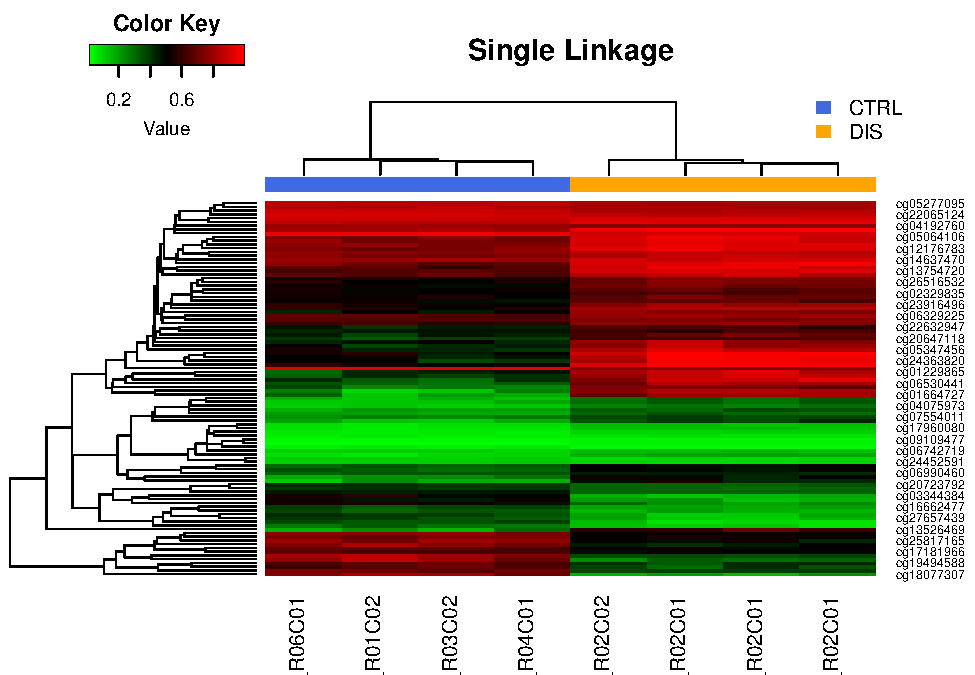
\includegraphics[keepaspectratio]{../results/HeatmapSingleLinkage-1.pdf}}

\textbf{Average linkage}

\begin{Shaded}
\begin{Highlighting}[]
\FunctionTok{heatmap.2}\NormalTok{(input\_heatmap,}
          \AttributeTok{col =}\NormalTok{ col2,}
          \AttributeTok{Rowv =} \ConstantTok{TRUE}\NormalTok{,}
          \AttributeTok{Colv =} \ConstantTok{TRUE}\NormalTok{,}
          \AttributeTok{hclustfun =} \ControlFlowTok{function}\NormalTok{(x) }\FunctionTok{hclust}\NormalTok{(x, }\AttributeTok{method =} \StringTok{"average"}\NormalTok{),}
          \AttributeTok{dendrogram =} \StringTok{"both"}\NormalTok{,}
          \AttributeTok{key =} \ConstantTok{TRUE}\NormalTok{,}
          \AttributeTok{ColSideColors =}\NormalTok{ colorbar,}
          \AttributeTok{density.info =} \StringTok{"none"}\NormalTok{,}
          \AttributeTok{trace =} \StringTok{"none"}\NormalTok{,}
          \AttributeTok{scale =} \StringTok{"none"}\NormalTok{,}
          \AttributeTok{symm =} \ConstantTok{FALSE}\NormalTok{,}
          \AttributeTok{main =} \StringTok{"Average Linkage"}\NormalTok{)}
\FunctionTok{legend}\NormalTok{(}\StringTok{"topright"}\NormalTok{, }\AttributeTok{legend =} \FunctionTok{c}\NormalTok{(}\StringTok{"CTRL"}\NormalTok{, }\StringTok{"DIS"}\NormalTok{), }\AttributeTok{fill =} \FunctionTok{c}\NormalTok{(}\StringTok{"royalblue"}\NormalTok{, }\StringTok{"orange"}\NormalTok{), }\AttributeTok{border =} \ConstantTok{NA}\NormalTok{, }\AttributeTok{bty =} \StringTok{"n"}\NormalTok{, }
       \AttributeTok{cex =} \FloatTok{0.8}\NormalTok{, }\AttributeTok{xpd =} \ConstantTok{TRUE}\NormalTok{, }\AttributeTok{inset =} \FunctionTok{c}\NormalTok{(}\DecValTok{0}\NormalTok{, }\SpecialCharTok{{-}}\FloatTok{0.10}\NormalTok{))}
\end{Highlighting}
\end{Shaded}

\pandocbounded{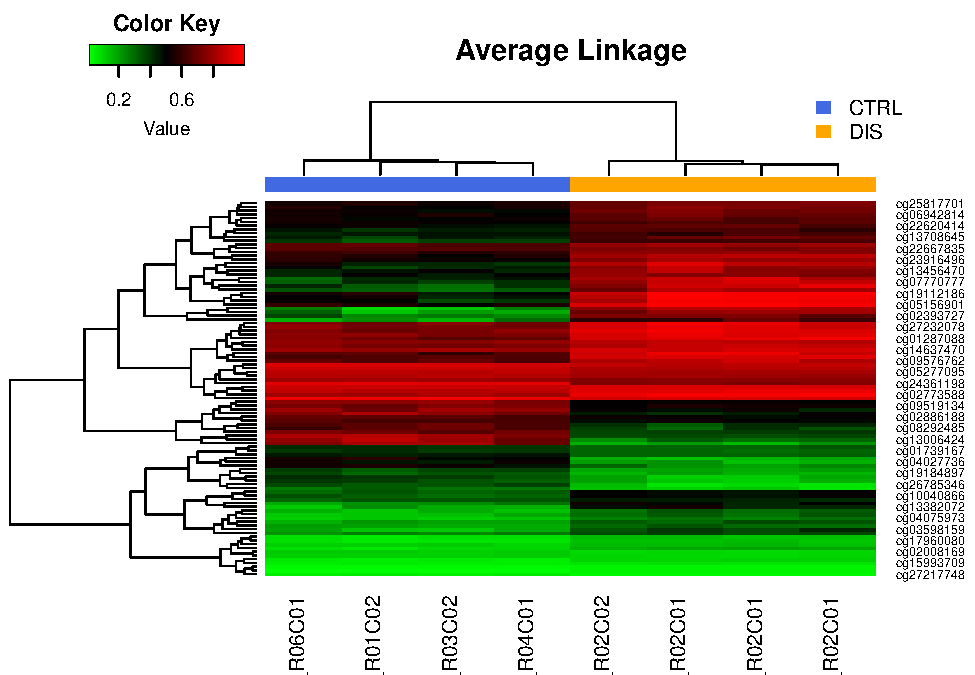
\includegraphics[keepaspectratio]{../results/HeatmapAvgLinkage-1.pdf}}

\end{document}
